% le caratteristiche richieste dall'università sono elencate qui: https://stem.elearning.unipd.it/mod/book/view.php?id=234&chapterid=46#modalita
% 12pt: font richiesto dall'università
% twoside: i margini interni ed esterni sono scambiati per le pagine "a sinistra" e "a destra"
% openright: i capitoli cominciano in pagine dispari ("a destra")
% extreport: supporta 12pt
\documentclass[12pt, a4paper, twoside, openright]{extreport}

% --- PACCHETTI ---

% margini
\usepackage{geometry}
\geometry{a4paper, top = 2cm, bottom = 2cm, outer = 2cm, inner = 3cm, includeheadfoot}

% unità di misura e matematica
\usepackage{siunitx, amsmath}
%\everydisplay{\footnotesize}
\everymath{\displaystyle}

% numerazione capitoli e formato titolo
\usepackage[english]{babel}
\usepackage{titlesec}
\titleformat{\chapter}[hang]                % titolo + numero sulla stessa linea
    {\normalfont\huge\bfseries}             % stile del titolo
    {\thechapter.}                          % numero del capitolo
    {1em}                                   % spazio tra numero e titolo
    {}                                      % codice prima del testo
\titlespacing*{\chapter}{0pt}{-10pt}{20pt}  % margini e spazi verticali



% didascalie
\usepackage{subcaption, caption}

% impaginazione
\usepackage{setspace}
\onehalfspacing
\setlength{\parindent}{0pt} % niente rientro nei paragrafi
\setlength{\parskip}{0.7em} % spazio tra paragrafi

\usepackage{enumitem}
\setlist{itemsep = 0.25em, topsep = 0.25em} % spazio tra elementi di una lista

\usepackage{tocloft} % 1. Carica il pacchetto
\setlength{\cftbeforechapskip}{20pt}

% font
\usepackage{times}

% colori, grafiche e tabelle
\usepackage[utf8]{inputenc}
\usepackage[T1]{fontenc}
\usepackage{booktabs}   % Per linee orizzontali professionali
\usepackage{longtable}  % Per tabelle che possono andare su più pagine
\renewcommand{\arraystretch}{1.3} % Aumenta leggermente lo spazio tra le righe
\usepackage[dvipsnames]{xcolor} % Per colori avanzati (opzionale, ma utile)
\usepackage{graphicx}
\usepackage{wrapfig}
\usepackage{tikz}
\usetikzlibrary{automata, positioning, arrows.meta, bending}
\usepackage{algorithm}
\usepackage{algpseudocode}
\usepackage{calc} % Serve per calcolare la larghezza della colorbox

% import/export formato pdf
\usepackage{pdfpages}
\usepackage[a-1a]{pdfx}
\hypersetup{hidelinks} % nascondi rettangoli di href

% bibliografia e appendice
\usepackage{csquotes, url}
\usepackage[backend = biber, style = ieee]{biblatex}
\addbibresource{bibliography.bib}
\usepackage[toc,page]{appendix}


% macro personalizzate

% --- PACCHETTI PER AMBIENTE TODO ---
\usepackage[breakable]{tcolorbox}

% --- DEFINIZIONE AMBIENTE TODO ---
% Crea un nuovo ambiente tcolorbox chiamato 'todo'
\newtcolorbox{todo}{
    colback   = red!5!white,  % Colore di sfondo (rosa = rosso 5% + bianco 95%)
    colframe  = red!75!black, % Colore del bordo (rosso scuro)
    fonttitle = \bfseries,    % Titolo in grassetto
    title     = {TODO:},      % Titolo automatico
    breakable = true,         % Permette al box di spezzarsi tra le pagine
    arc       = 2mm,          % Angoli leggermente arrotondati
    boxrule   = 0.5mm,        % Spessore del bordo
}

% --- MACRO PER SEGNAPOSTO IMMAGINE ---
% Crea un box segnaposto per una figura
% Argomenti:
% #1: label (per \ref)
% #2: didascalia (per \caption)
% #3: Testo principale (grassetto)
% #4: Descrizione (corsivo)
\newcommand{\segnaposto}[4]{%
    \begin{figure}[htbp]
    \centering
    \framebox{\parbox{0.6\textwidth}{\centering
        \vspace{3cm} % Spazio sopra
        \textbf{#3} \\
        \small\textit{#4}
        \vspace{3cm} % Spazio sotto
    }}
    \caption{#2}
    \label{#1}
    \end{figure}
}

% --- DEFINIZIONE MACRO PER I BLOCCHI COLORATI ---
% Sintassi: \ColorBlock{ColoreSfondo}{Contenuto}
\newcommand{\ColorBlock}[2]{%
    \State \makebox[\linewidth][l]{%
        \colorbox{#1!15}{% !15 rende il colore molto tenue (pastello)
            \parbox{\dimexpr\linewidth-2\fboxsep}{#2}%
        }%
    }%
}

% --- DOCUMENTO PRINCIPALE ---

% --- FRONTESPIZIO ---
\title{Hardware/Software Design and Implementation\\of an Open Robotic Chain\\Using Custom Servo-Motor Modules}
\author{Gottardo Filippo}
\date{04/12/2025}
\newcommand{\supervisor}{Prof. Cenedese Angelo}
\newcommand{\cosupervisor}{Ing. Antonello Riccardo}

% inizio del documento
\begin{document}
    \pagenumbering{Roman}
    \pagestyle{empty}
    \input{chapters/ch0/frontespizio.tex}
    \pagestyle{plain}
    \cleardoublepage

    % --- ABSTRACT ---
    \chapter*{Abstract}
\addcontentsline{toc}{chapter}{Abstract}

This thesis presents a comprehensive, top-down engineering approach to the design and control of a modular robotic
limb for a hexapod platform. The primary objective is to overcome the performance limitations inherent in low-cost
commercial actuation, which typically hinder precise legged locomotion.

The research begins with the kinematic modeling and digital simulation of the limb in the MATLAB/Simulink environment,
establishing a simulation model to validate trajectory planning and inverse kinematics algorithms. The core contribution
of this work is the development of a novel, custom "Smart Actuator" module designed to replace standard hobbyist
servo-motors. This custom embedded solution integrates a high-resolution magnetic encoder, a high-current H-bridge
driver, and an STM32 microcontroller. Crucially, it implements a non-linear Switching PID control strategy specifically
tuned to mitigate stick-slip friction phenomena and mechanical backlash.

The system is validated through a Hardware-in-the-Loop (HIL) architecture, bridging the simulation environment with the
physical prototype. Experimental benchmarking demonstrates a dramatic improvement in performance.

    % --- INDICE ---
    \cleardoublepage
    \tableofcontents
    \cleardoublepage
    \pagenumbering{arabic}
    %\chapter{Introduction}

\chapter{Methodologies, Design and Simulation}
    \section{Mechanical Design}
        \subsection{Denavit--Hartenberg Overview}
        \subsection{Limb Parametrization and Forward Kinematics}
        \subsection{Inverse Kinematics Overview and Derivation}
    \section{Workspace and Path Planning}
        \subsection{Workspace Definition and Analysis}
        \subsection{Trajectory Design}
    \section{Control and Simulation}
        \subsection{Open Loop Control Strategy}
        \subsection{Digital Simulation Setup}
        \subsection{Results}
    \section{Proprioception and Path Adaptation}
        \subsection{Contact Sensing and Architectuaral Shift}
        \subsection{Finite State Trajectory Generator}
        \subsection{Adaptive Simulation Results}

\chapter{Custom Smart Actuator Module Design}
    \section{Limitations of Commercial Servos}
    \section{Hardware Design and Component Selection}
        \subsection{Requirements Definition}
        \subsection{Components Selection}
        \subsection{PCB Design and Layout}
    \section{Embedded Software Architecture}
        \subsection{Control Strategy}
    \section{Module Characterization and Benchmarking}
        \subsection{Static Analysis: Linearity and Hysteresis}
        \subsection{Step Response Analysis: Response and Precision}
        \subsection{Results Summary}

\chapter{Prototype Implementation}
    \section{Hardware-in-the-Loop Architecture}
        \subsection{Limb Assembly}
        \subsection{Simulink Setup}
        \subsection{Arduino Setup}
    \section{Performance Assessment}

\chapter{Conclusions}
    \section{Achievements and Considerations}
    \section{Economical and Practical Aspects}
    \section{General Applicability and Future Work}

\chapter{Acknowledgements}
    \section{AI Fair Use}
    \section{Ringraziamenti}

% --- Appendices ---
\appendix
\chapter{Appendix}

% --- Bibliography ---
\addcontentsline{toc}{chapter}{Bibliography}

\begin{thebibliography}{99}

\end{thebibliography}     % mockup del contenuto

    % --- CAPITOLI ---
    \chapter{Introduction}

The field of bio-inspired robotics \cite{delcomyn2004insect} has seen rapid advancements in recent years,
\cite{chai2022survey,fan2024review} driven by the need for autonomous systems capable of navigating
unstructured and complex environments. Among these, hexapod robots offer a unique combination of stability,
payload capacity, and terrain adaptability that wheeled platforms cannot match. However, the effective deployment
of such legged systems is fundamentally dictated by the quality of their actuation.


\subsubsection{Motivation and Problem Statement}

Precise legged locomotion requires accurate control of joint angles and torque. While industrial-grade actuators
(e.g. Dynamixel-X series \cite{robotis_dynamixel_x}) offer the necessary fidelity and communication interfaces,
their prohibitive cost makes them inaccessible for many research and prototyping applications. Conversely,
low-cost "hobby" servo-motors, while affordable, present critical limitations. They typically operate as
"black boxes" with inaccessible internal control loops, rely on wear-prone resistive potentiometers for feedback,
and suffer from significant deadbands and non-linear friction effects.


\subsubsection{Thesis Objectives}

This thesis addresses these challenges by proposing a comprehensive hardware-software design. The overarching goal
is to bridge the gap between low-cost hardware and high-performance control. The specific objectives are:

\begin{enumerate}
    \item \textbf{Kinematic Framework:} To derive and validate the mathematical model of a 3-DOF hexapod limb,
        ensuring reliable workspace analysis and trajectory planning.
    \item \textbf{Actuator Redesign:} To engineer a custom "Smart Actuator" module that retains the standard form factor
        of commercial servos but upgrades performances through internal electronics replacements.
    \item \textbf{Sim-to-Real Validation:} To establish a Hardware-in-the-Loop (HIL) architecture that allows for direct
        performance comparison between a theoretical numerical model and the physical prototype.
    \item \textbf{Modular Scalability:} To adopt a strictly modular design philosophy for both hardware and software
        architectures, ensuring that the single-leg system can be seamlessly replicated and integrated to realize the
        complete hexapod robot in future developments.
\end{enumerate}


\subsubsection{Thesis Structure}

The remainder of this thesis is organized as follows:

\begin{itemize}
    \item Chapter \ref{ch:model} establishes the theoretical foundation. It details the mechanical design of the limb,
        the Denavit--Hartenberg parameterization, and the Inverse Kinematics derivation. It also presents the
        numerical model developed in Simscape Multibody, which serves as reference for validation.
    \item Chapter \ref{ch:servomotor} focuses on the component-level engineering. It analyzes the limitations of
        commercial servos and details the hardware and software design of the custom actuator module, including the
        Switching PID control algorithm, ultimately evaluating the achieved improvements.
    \item Chapter \ref{ch:prototype} describes the system integration and experimental validation. It outlines the
        Hardware-in-the-Loop architecture and presents a quantitative comparison of the trajectory tracking performance
        between the simulation and the physical prototype.
    \item Chapter \ref{ch:conclusions} concludes the thesis by summarizing the achieved results, and outlining future
        research directions.
\end{itemize}


    \chapter{Model Design and Simulation}
\label{ch:model}

This chapter illustrates the theoretical steps of design, control and simulation of the robotic system. The analysis
deliberately focuses on the developement of a single leg of a hexapod robot.

This strategic choice adheres to a modular approach, which is convenient for several reasons.
Firstly, it ensures that the design can be easily extended and replicated for the remaining limbs, simplifying
the eventual future assembly of the complete robot. Secondly, isolating the study to a single leg allows for a
concentrated focus on the fundamental kinematic and control aspects, thereby optimizing the analysis and
limiting system complexity and implementation time.

\section{Structural Design}

The robotic leg is conceived as a three degrees of freedom (3-DOF) manipulator, a common simplification
of an insect's limb, designed to provide sufficient motion versatility within a robust and manageable structure.
The kinematic chain consists of three rigid links — Coxa, Femur, and Tibia — connected sequentially by three
revolute joints (from the robot's body toward the end-effector, as shown in Figure \ref{fig:hexapod_leg}):

\begin{itemize}
    \item \textbf{Hip Joint} ($q_1$): Connects the robot's body to the Coxa link and primarily controls the
        \textbf{yaw} motion of the leg, responsible for the lateral sweep relative to the body's longitudinal axis.
    \item \textbf{Knee Joint} ($q_2$): Connects the Coxa link to the Femur link and controls the
        \textbf{primary pitch} motion, enabling the lifting and lowering of the leg structure.
    \item \textbf{Ankle Joint} ($q_3$): Connects the Femur link to the Tibia link and controls the
        \textbf{secondary pitch} motion, significantly influencing the height and reach of the Foot (end-effector).
\end{itemize}

This configuration, is widely adopted in hexapod designs as it provides an optimal balance between complexity
and dexterity, allowing for effective gait planning and stable locomotion on various surfaces.

\begin{figure}[htbp]
    \centering
    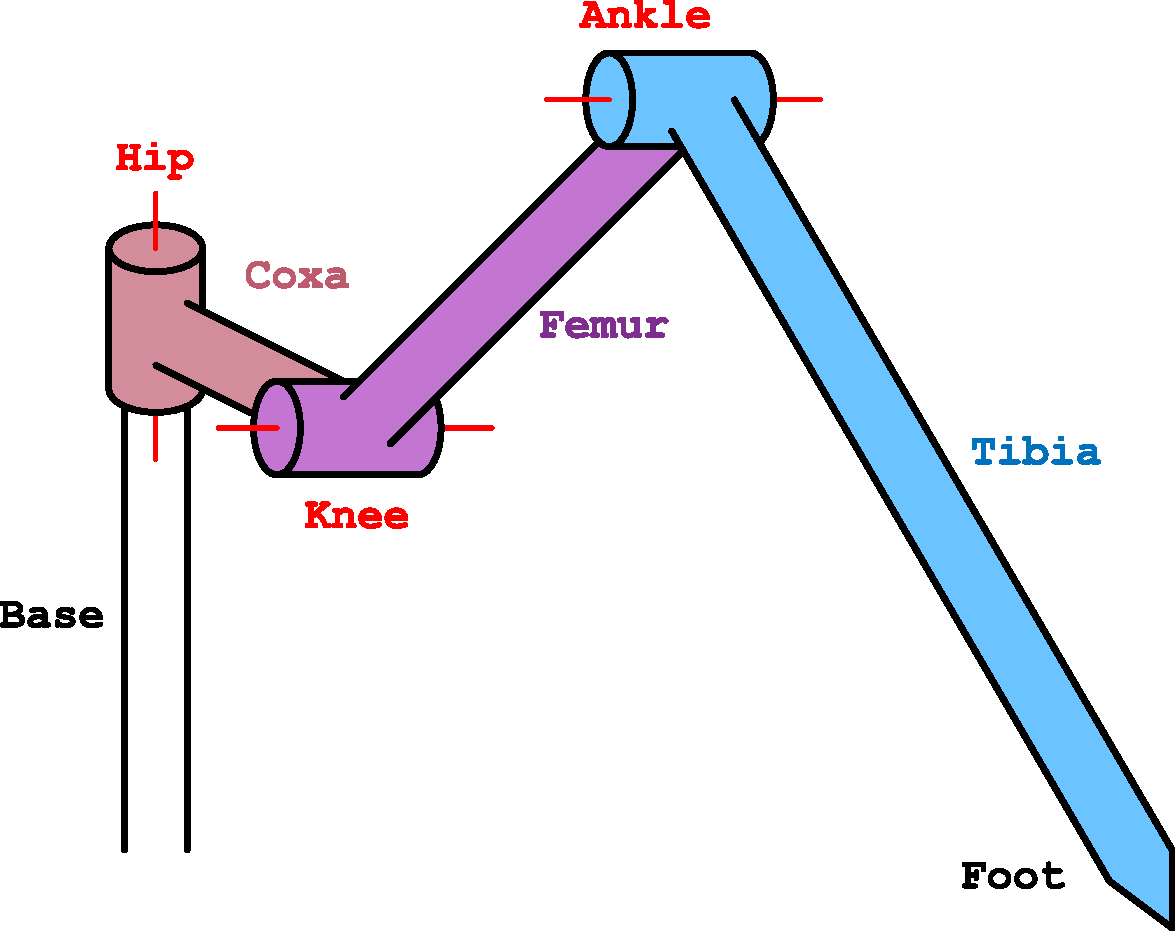
\includegraphics[width=0.8\textwidth]{images/hexapod-leg.pdf}
    \caption{Schematic Representation of the Mechanical Limb}
    \label{fig:hexapod_leg}
\end{figure}


\subsection{Limb Parametrization and Forward Kinematics}
\label{sec:dh_params}

The Denavit--Hartenberg (DH) convention \cite{denavit1955kinematic, siciliano2009robotics} is the standard
mathematical tool for describing the spatial relationships and defining the minimal parameter set required for
kinematic analysis of serial manipulators. By rigidly attaching coordinate frames to each link, DH enables a
standardized description of the link geometry and joint configuration.

The assignment of these frames follows a systematic methodology designed to isolate the four key parameters.
For a kinematic chain starting from a base frame $\{0\}$, a coordinate frame $\{i\}$ is rigidly attached to
link $i$. The most important rule is that the $z_i$-axis is placed along the axis of actuation (either
rotation or translation) for joint $i$. The $x_i$-axis is then constructed along the common normal connecting
$z_{i-1}$ (the previous joint axis) to $z_i$ (the current joint axis), with the origin of frame $\{i\}$
located at the intersection of $x_i$ and $z_i$. Finally, the $y_i$ axis is simply set to complete a
right-handed coordinate system.

Using this precise, rule-based placement of axes the entire transformation from frame $\{i\}$ to frame $\{i+1\}$
can now be described by a sequence of four fundamental operations tied directly to this geometry: the Link Length
($a_i$), Link Twist ($\alpha_i$), Link Offset ($d_i$), and the Joint Angle ($\theta_i$) (see Figure
\ref{fig:denavit_hartenberg}).

\begin{figure}[htbp]
    \centering
    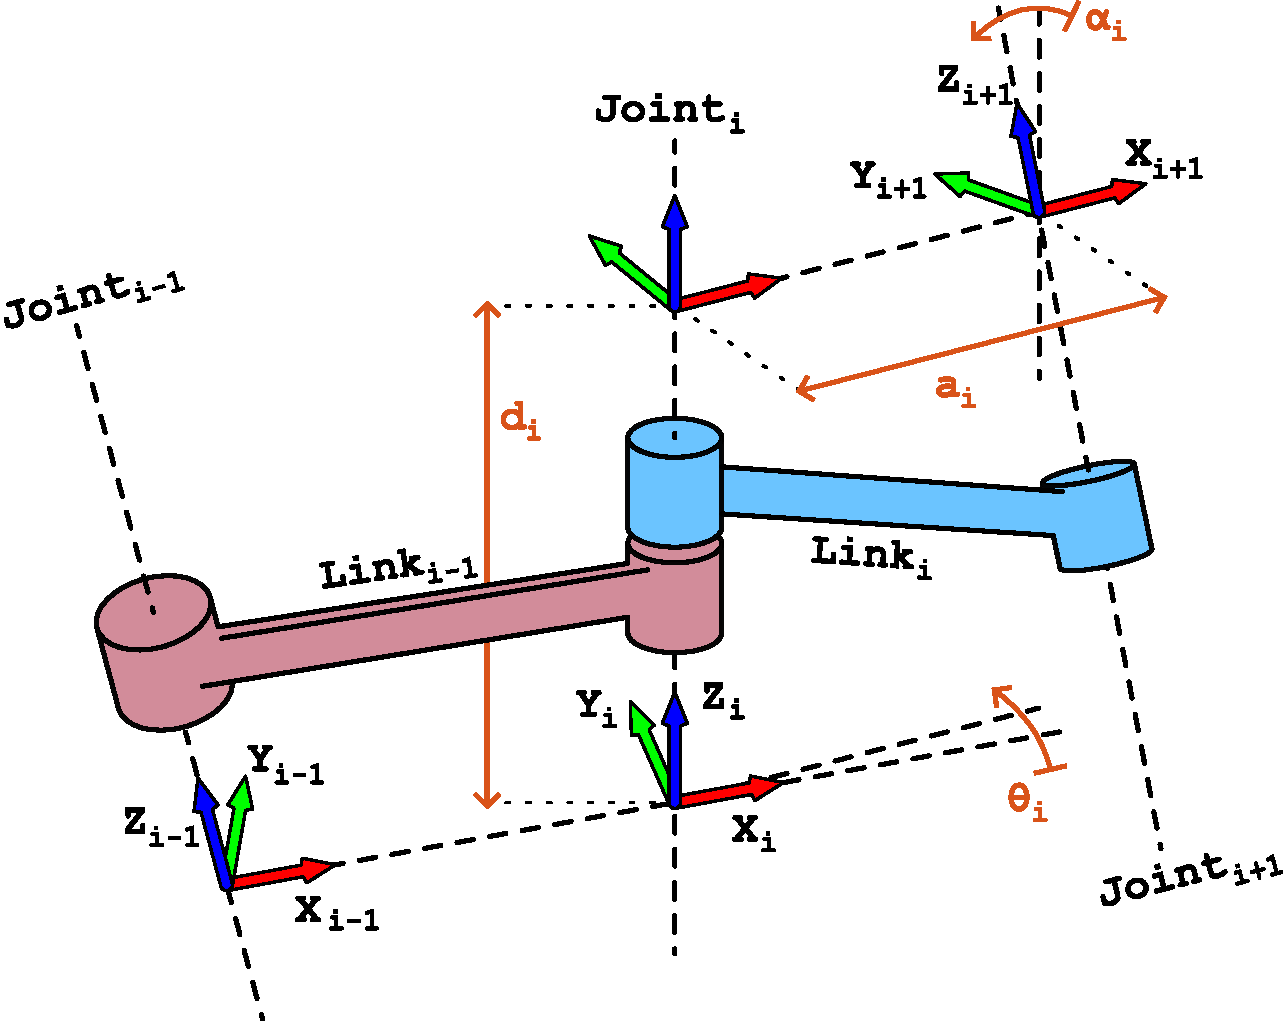
\includegraphics[width=0.8\textwidth]{images/denavit-hartenberg.pdf}
    \caption{Illustration of Denavit--Hartenberg Convention Parameters}
    \label{fig:denavit_hartenberg}
\end{figure}

The homogeneous transformation matrix, $T_{i}^{i+1}$, from frame $\{i\}$ to frame $\{i+1\}$, is given by:

\begin{equation}
    T_{i}^{i+1} = R_x(\alpha_i) \cdot T_x(a_i) \cdot R_z(\theta_i) \cdot T_z(d_i) =
    \begin{bmatrix}
        c_{\theta} & -s_{\theta} & 0 & a \\
        s_{\theta} c_{\alpha} & c_{\theta} c_{\alpha} & -s_{\alpha} & -ds_{\alpha} \\
        s_{\theta} s_{\alpha} & c_{\theta} s_{\alpha} & c_{\alpha} & dc_{\alpha} \\
        0 & 0 & 0 & 1
    \end{bmatrix}
\end{equation}

where the contracted notation $c_x = \cos(x), s_x = \sin(x)$ was used, while the overall transformation from
the base frame $\{b\}$ to the end-effector frame $\{e\}$, $T_b^e$, which is the Forward Kinematics solution,
is computed by the serial multiplication of these individual matrices:

\begin{equation}
    T_b^e = T_b^1 T_1^2 \dots T_{n-1}^n T_n^e
    \label{eqn:transf_matrix}
\end{equation}

To formally derive the Forward Kinematic model of the 3-DOF robotic limb, we apply the DH convention, following
the methodology introduced in the previous section. The assignment of the reference frames is shown in Figure
\ref{fig:assign_dh}, where the $z$-axes are represented in blue, $x$-axes in red and the $y$-axes are omitted.

Frame $\{b\}$ serves as the fixed base frame. In the context of a complete mobile hexapod, this frame is
typically attached to the center of the robot's main body to facilitate gait planning relative to the body's
center of gravity. However, for the experimental verification of the single modular limb in a benchtop setup,
frame $\{b\}$ is rigidly attached to the stationary mounting base, establishing a fixed reference for all
subsequent transformations.

\begin{figure}[htbp]
    \centering
    \begin{subfigure}[c]{0.48\textwidth}
        \centering
        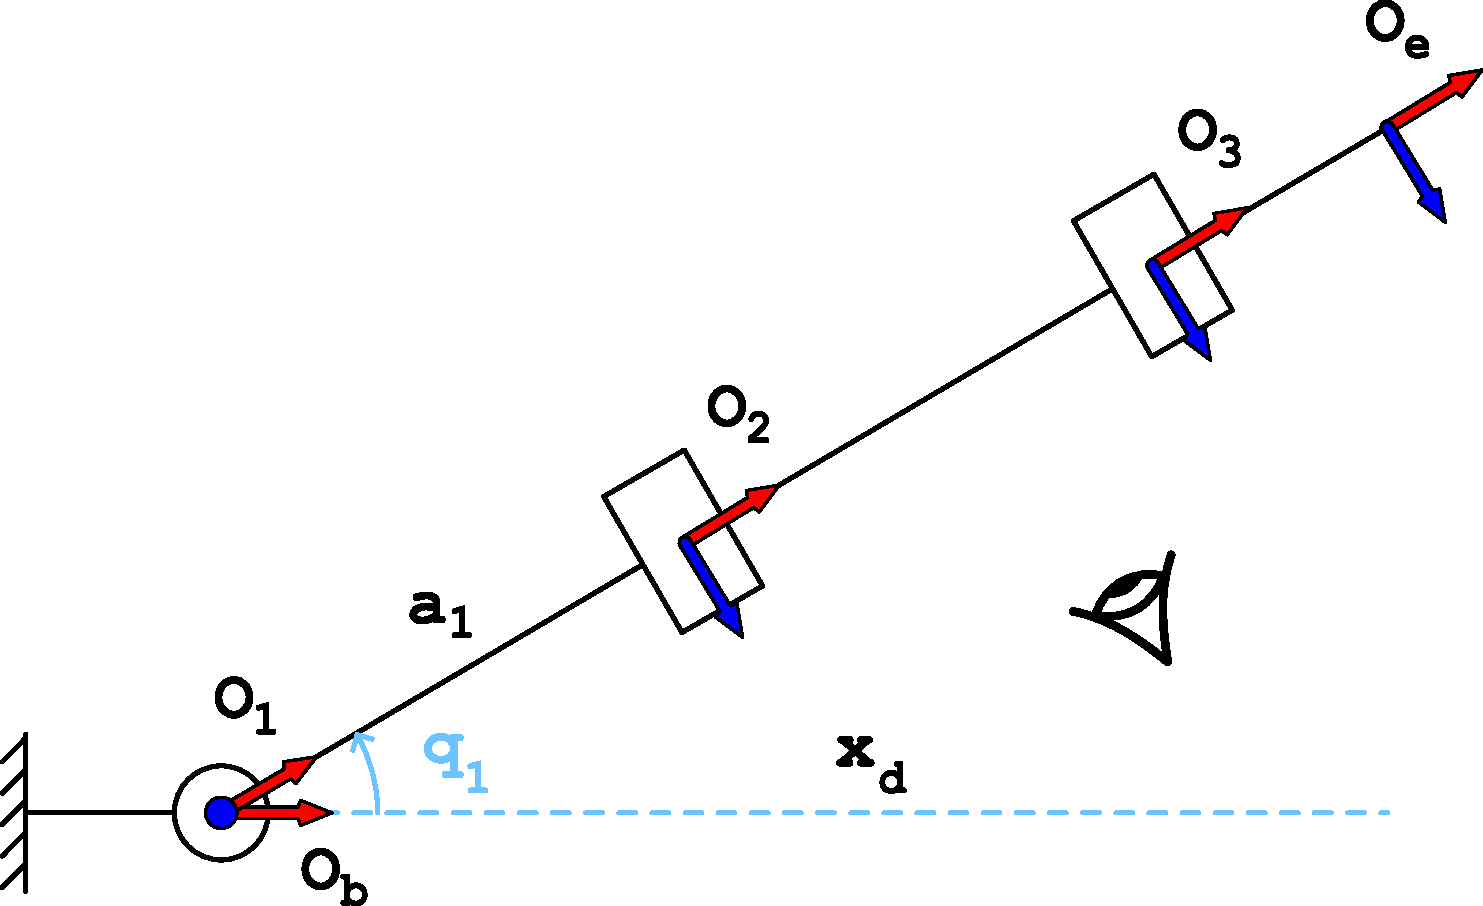
\includegraphics[width=\textwidth]{images/leg-top-dh.pdf}
        \caption{Top View}
        \label{fig:dh_top}
    \end{subfigure}
    \hfill
    \begin{subfigure}[c]{0.48\textwidth}
        \centering
        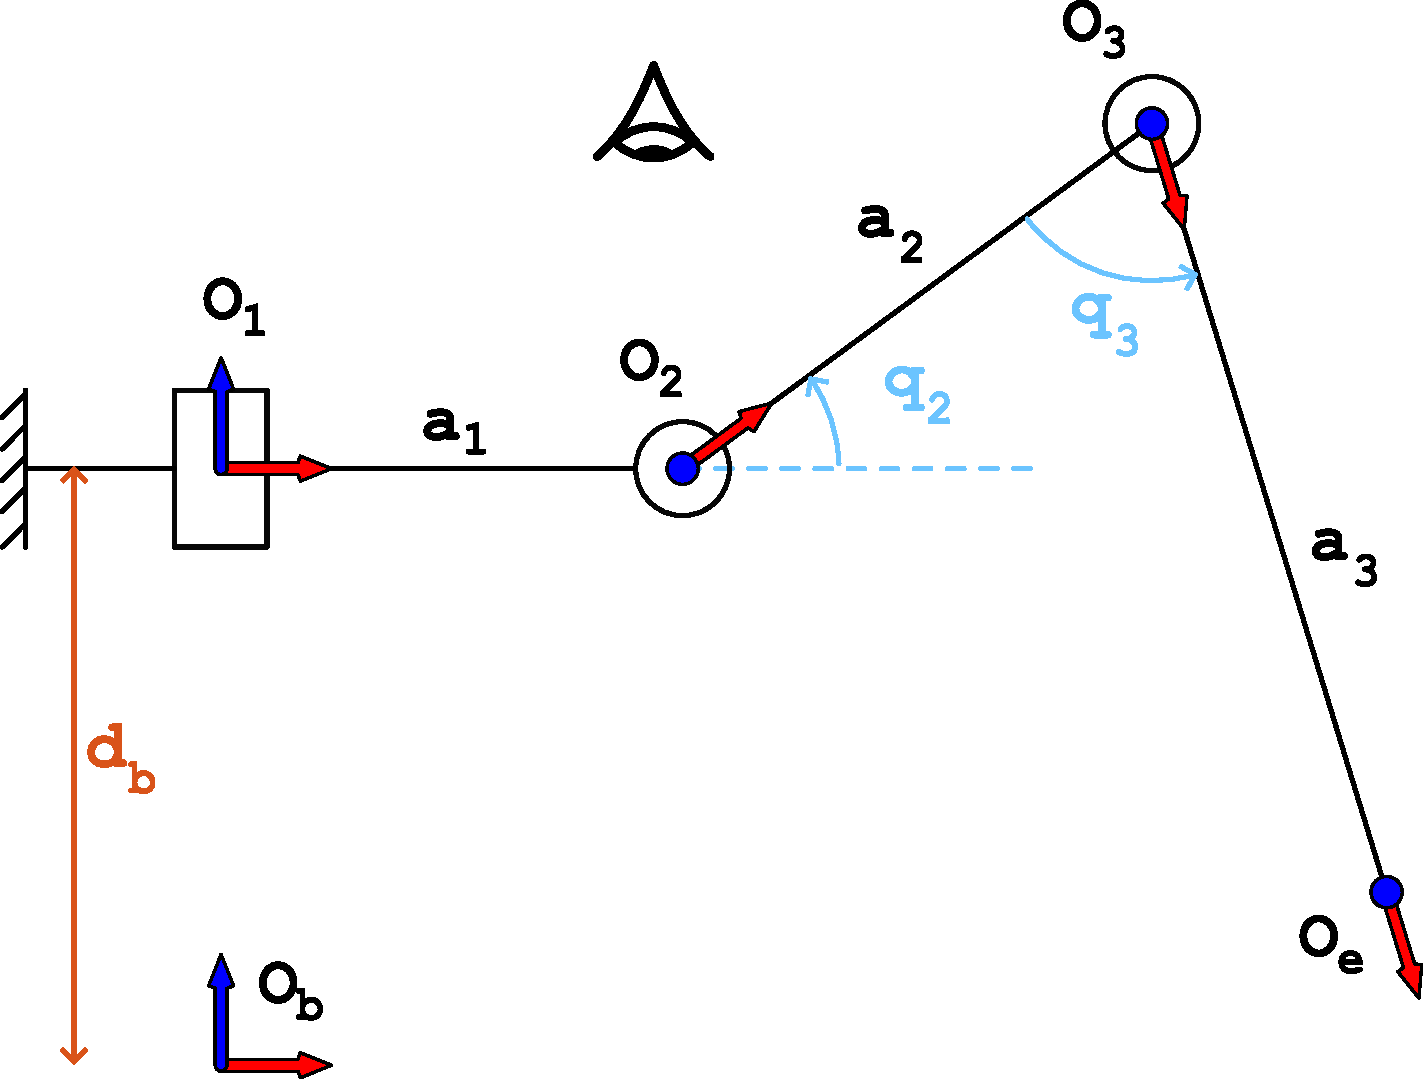
\includegraphics[width=\textwidth]{images/leg-side-dh.pdf}
        \caption{Side View}
        \label{fig:dh_side}
    \end{subfigure}
    \caption{Reference Frames and DH Parameters}
    \label{fig:assign_dh}
\end{figure}

Note the following key design choices:

\begin{itemize}
    \item The base offset $d_b$ represents the distance from the base frame $\{b\}$ to the frame of the Hip Joint
        (i.e. the mounting height of the leg on the base).
    \item The link lengths $a_1$, $a_2$ and $a_3$ correspond to the length of the Coxa, Femur and Tibia links,
        respectively. These values are chosen based on a mix of aesthetics and physical constraints. More
        specifically, the Coxa length is minimized and the Femur length is chosen to be smaller than the Tibia
        length.
    \item The twist angle $\alpha_1 = 90^{\circ}$ is necessary because the axis of the Knee Joint ($z_2$) is
        orthogonal to the axis of the Hip Joint ($z_1$).
    \item Subsequent frames are coplanar, resulting in zero twist angles ($\alpha_2 = \alpha_3 = 0^{\circ}$)
        and link offsets ($d_1 = d_2 = d_3 = 0\ mm$), simplifying the transformation matrices.
    \item The joint angle $q_3$ is rotated by an extra $-180^\circ$ to simplify IK derivation and match the
        hardware implementation.
    \item Since the attitude of the end-effector is irrelevant, the final joint angle for the Tibia link is
        fixed at $\theta_4 = 0$, as the end-effector (Foot) frame $\{e\}$ is placed at the tip of the Tibia
        link, defining the final link length $a_3$.
\end{itemize}

The parameter for the DH model are reported in Table \ref{tab:dh_parameters}.

\begin{table}[htbp]
    \centering
    \begin{tabular}{c c c c c}
        \hline
        \textbf{Link} & \textbf{$a$ [mm]} & \textbf{$\alpha$ [deg]} & \textbf{$d$ [mm]} & \textbf{$\theta$ [deg]} \\
        \hline
        \hline
        Base    & $0$           & $0$   & $d_b = 178$   & $q_1$         \\
        Coxa    & $a_1 = 40$    & $90$  & $0$           & $q_2$         \\
        Femur   & $a_2 = 78$    & $0$   & $0$           & $q_3 - 180$   \\
        Tibia   & $a_3 = 132$   & $0$   & $0$           & $0$           \\
        \hline
    \end{tabular}
    \caption{Denavit--Hartenberg Parameters of the Limb}
    \label{tab:dh_parameters}
\end{table}


\subsection{Inverse Kinematics Overview and Derivation}

Forward Kinematics analysis allows for the straightforward computation of the end-effector's pose starting from a
known joint configuration. However, this direct mapping is often impractical for high-level control. Defining a
task or a trajectory is inherently more intuitive in Cartesian space (e.g. coordinates in the world frame) than
in the abstract joint space. Consequently, to command the robot to reach a specific physical location, the
inverse problem must be addressed.

Inverse Kinematics (IK) \cite{siciliano2009robotics} is the problem of determining the set of joint variables,
$q = [q_1, \dots, q_n]$, required to place the end-effector at a desired pose, $p_d = [x_d, y_d, z_d, \phi_d, \theta_d, \psi_d]^T$.
Unlike Forward Kinematics, the IK problem is fundamentally more challenging due to the non-linear relationship
between joint space and Cartesian space. The mathematical objective is to solve the inverse mapping:
\begin{equation*}
    q = f^{-1}(p_d)
\end{equation*}

The complexity of the problem stems from several factors. Solutions may be non-unique, meaning multiple
joint configurations can achieve the same end-effector pose and/or non-existent if the target pose lies outside
the robot's physical workspace. Furthermore, singularities — joint configurations that cause a loss of effective
degrees of freedom — must be avoided as they lead to control instability.

To address these challenges, solution approaches usually fall into two main categories: on one side, analytical
solutions provide closed-form, explicit equations for the joint variables as a function of the desired pose,
offering high computational efficiency and usually providing all possible solutions. They are generally preferred
for manipulators with simple geometries. Numerical Methods, conversely, use iterative algorithms to converge on a
solution by minimizing a position error function. While they are necessary for complex kinematic structures
lacking analytical solutions, they are less computationally efficient and provide only one solution per iteration.

Given the simple structure of the application, an analytical solution can be found using planar geometry and
fundamental trigonometric relationships. For the derivation, the leg geometry is conceptually separated into two
different point of views, to facilitate the calculation. Figure \ref{fig:find_ik} depicts a schematic representation
of them.

\begin{figure}[htbp]
    \centering
    \begin{subfigure}[t]{0.48\textwidth}
        \centering
        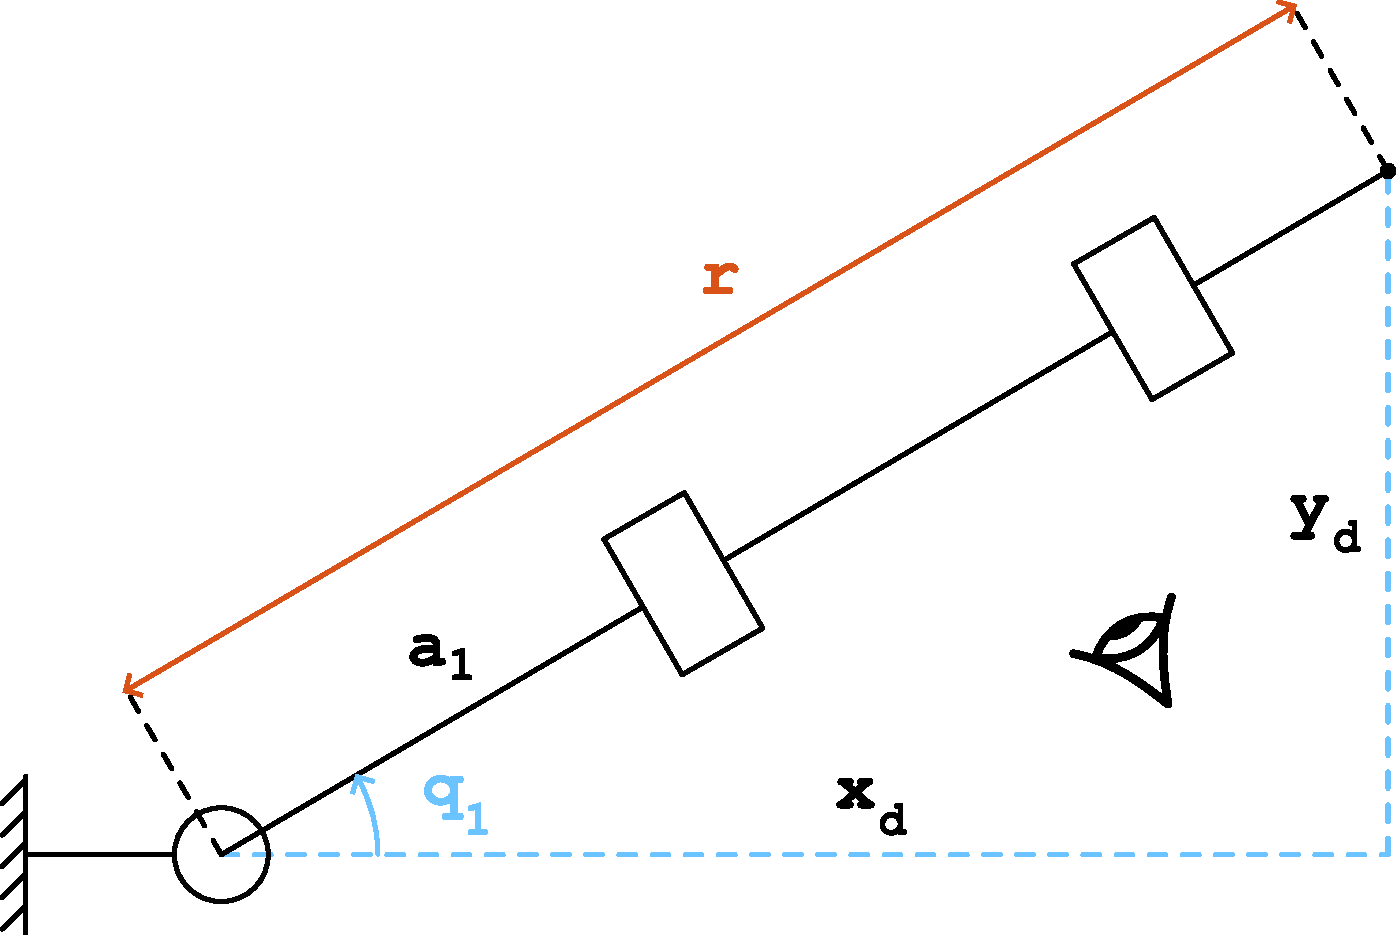
\includegraphics[width=\textwidth]{images/leg-top-ik.pdf}
        \caption{Top View}
        \label{fig:ik_top}
    \end{subfigure}
    \hfill
    \begin{subfigure}[t]{0.48\textwidth}
        \centering
        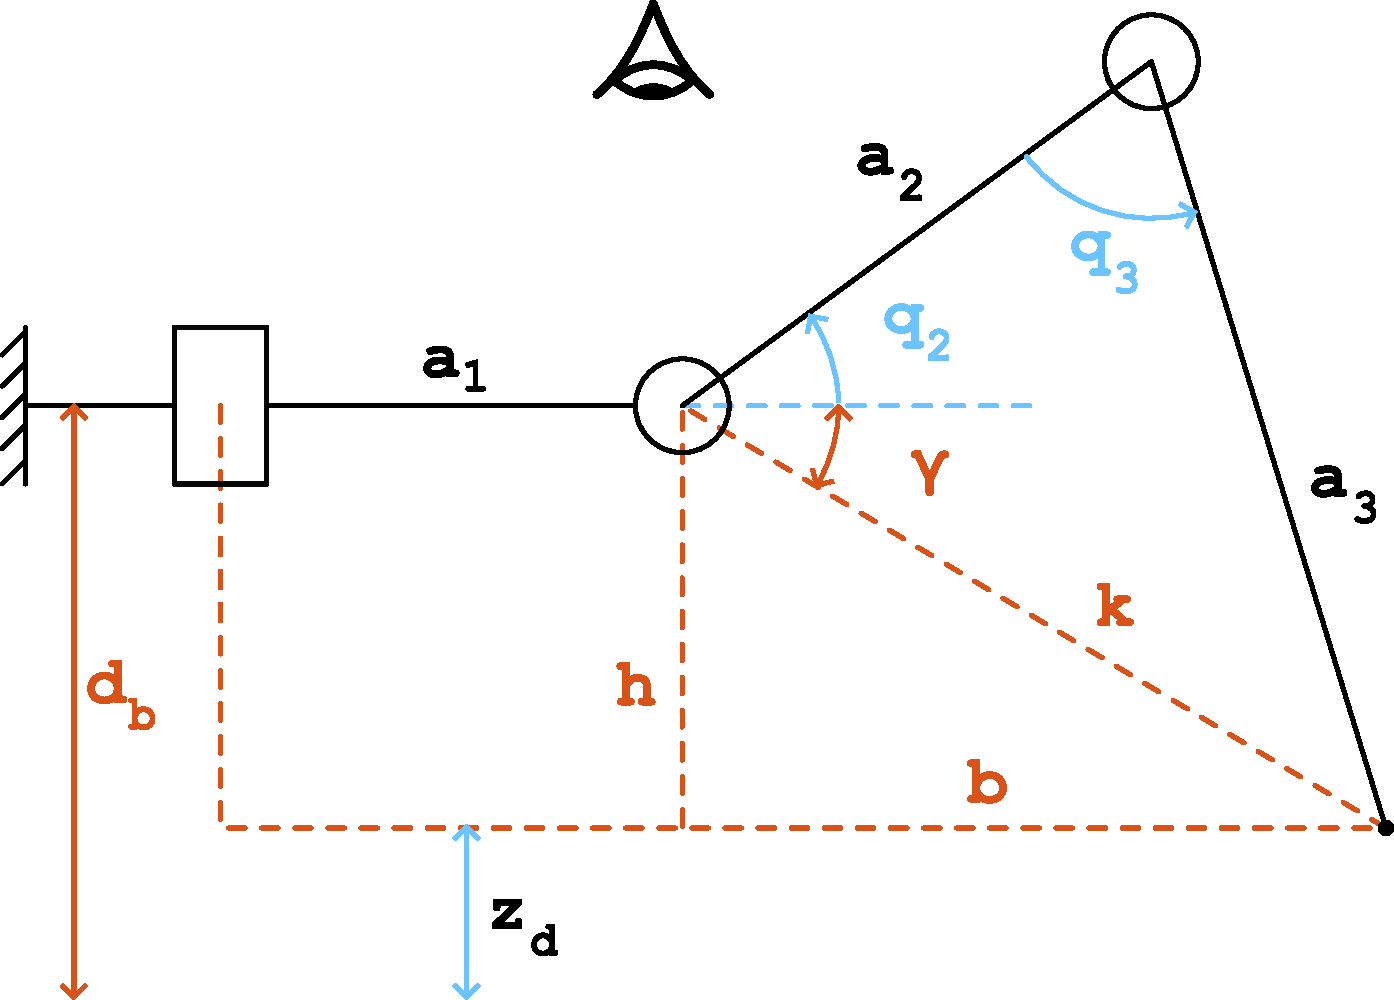
\includegraphics[width=\textwidth]{images/leg-side-ik.pdf}
        \caption{Side View}
        \label{fig:ik_side}
    \end{subfigure}
    \caption{Leg Geometry for IK Derivation}
    \label{fig:find_ik}
\end{figure}

Given a desired end-effector position $p_d = [x_d, y_d, z_d]^T$, the three required joint angles $q_1, q_2, q_3$
can be determined sequentially as follows:


\subsubsection{Joint Angle $q_1$ (Yaw)}

The first joint angle, $q_1$, is determined solely by the $X$ and $Y$ coordinates of the desired position,
representing a rotation in the horizontal plane (Figure \ref{fig:ik_top}). This is a straightforward calculation:
\begin{equation*}
    q_1 = \operatorname{atan2}(y_d,x_d)
\end{equation*}
The $\operatorname{atan2}$ function ensures that the resulting angle correctly accounts for the sign of the
coordinates across all four quadrants, providing the correct angle $\theta \in [-\pi, \pi]$.


\subsubsection{Joint Angles $q_2$ and $q_3$ (Pitch)}

The derivation of $q_2$ and $q_3$ is performed in the vertical plane (Figure \ref{fig:ik_side}),
which is defined by the Femur and Tibia links. We first define a set of auxiliary geometric variables:
\begin{itemize}
    \item \textbf{Projected Radial Distance ($r$):} The distance from the origin to the end-effector projected
        onto the $XY$-plane.
        \begin{equation*}
            r = \sqrt{x_d^2 + y_d^2}
        \end{equation*}
    \item \textbf{Horizontal Distance ($b$):} The effective horizontal distance from the $q_2$ joint axis to
        the end-effector.
        \begin{equation*}
            b = r - a_1 \Leftarrow r = b + a_1
        \end{equation*}
    \item \textbf{Vertical Distance ($h$):} The effective vertical distance from the $q_2$ joint axis to
        the end-effector.
        \begin{equation*}
            h = d_b - z_d
        \end{equation*}
    \item \textbf{Virtual Link Length ($k$):} The length of the virtual link connecting the $q_2$ joint axis
        to the end-effector, forming the third side of the triangle with links $a_2$ and $a_3$.
        \begin{equation*}
            k = \sqrt{h^2 + b^2}
        \end{equation*}
    \item \textbf{Knee Offset Angle ($\gamma)$:} The angle between the continuation of $a_1$ and the
        virtual link length $k$.
        \begin{equation*}
            \gamma = \operatorname{atan2}(h, b)
        \end{equation*}
        Using $\operatorname{atan2}$ ensures once again correctness even when $h$ is negative, i.e. when the
        Foot is above the body of the robot.
\end{itemize}

Using these auxiliary variables, the final joint angles $q_2$ and $q_3$ can now be obtained.

The second joint angle, $q_2$, is found by determining the internal angle of the $a_2, a_3, k$ triangle
using the Law of Cosines and compensating for the angle ($\gamma$):
\begin{equation*}
    q_2 = \operatorname{acos}\left(\frac{a_2^2 + k^2 - a_3^2}{2 \cdot a_2 \cdot k}\right) - \gamma
\end{equation*}
The third and final joint angle, $q_3$, is the angle between the $a_2$ and $a_3$ links. This is again derived
from the Law of Cosines:
\begin{equation*}
    q_3 = \operatorname{acos}\left(\frac{a_2^2 + a_3^2 - k^2}{2 \cdot a_2 \cdot a_3}\right)
\end{equation*}

Substituting the intermediate variables back into the expressions for $q_2$ and $q_3$ yields the final,
consolidated IK equations as a direct function of the desired end-effector coordinates as reported in Appendix
\ref{app:ik}.

\section{Reachable Workspace and Path Planning}
\label{sec:trajectory}

Following the developement of the limb's kinematic model, the next logical step is to verify the correctness of
the design and its behaviour through digital simulation. However, two preliminary steps are essential: the reachable
workspace of the system must be analyzed to understand its operational boundaries and a desired trajectory for the
end-effector must be designed.


\subsection{Workspace Definition and Analysis}

The reachable workspace of a manipulator is formally defined as the complete set of all Cartesian positions
$p = [x,y,z]^{T}$ that its end-effector can attain, given the physical constraints of its kinematic
chain \cite{ding2010locomotion}. It represents the entire volume of space accessible to the robot's
end-effector. For this 3-DOF limb, the workspace is determined by the three link lengths ($a_{1},a_{2},a_{3}$)
and, most critically, by the actuation limits imposed on its three joints ($q_{1},q_{2},q_{3}$).

To characterize this 3D volume, a two-stage approach is taken. First, the 2D planar workspace is analyzed.
This is done by fixing the Hip Joint at a neutral angle (e.g. $q_1 = \ang{0}$) and generating the boundary of
the leg's reach in a single vertical plane. A 2D cross-section is then obtained by sweeping the Knee
($q_2$) and Ankle ($q_3$) joints through their entire operational ranges. The resulting surface (Figure
\ref{fig:workspace_analysis}) is finally revolved around the Hip joint axis by sweeping $q_1$ through its own
range, thereby generating the final 3D reachable volume.

\begin{figure}[htbp]
    \centering
    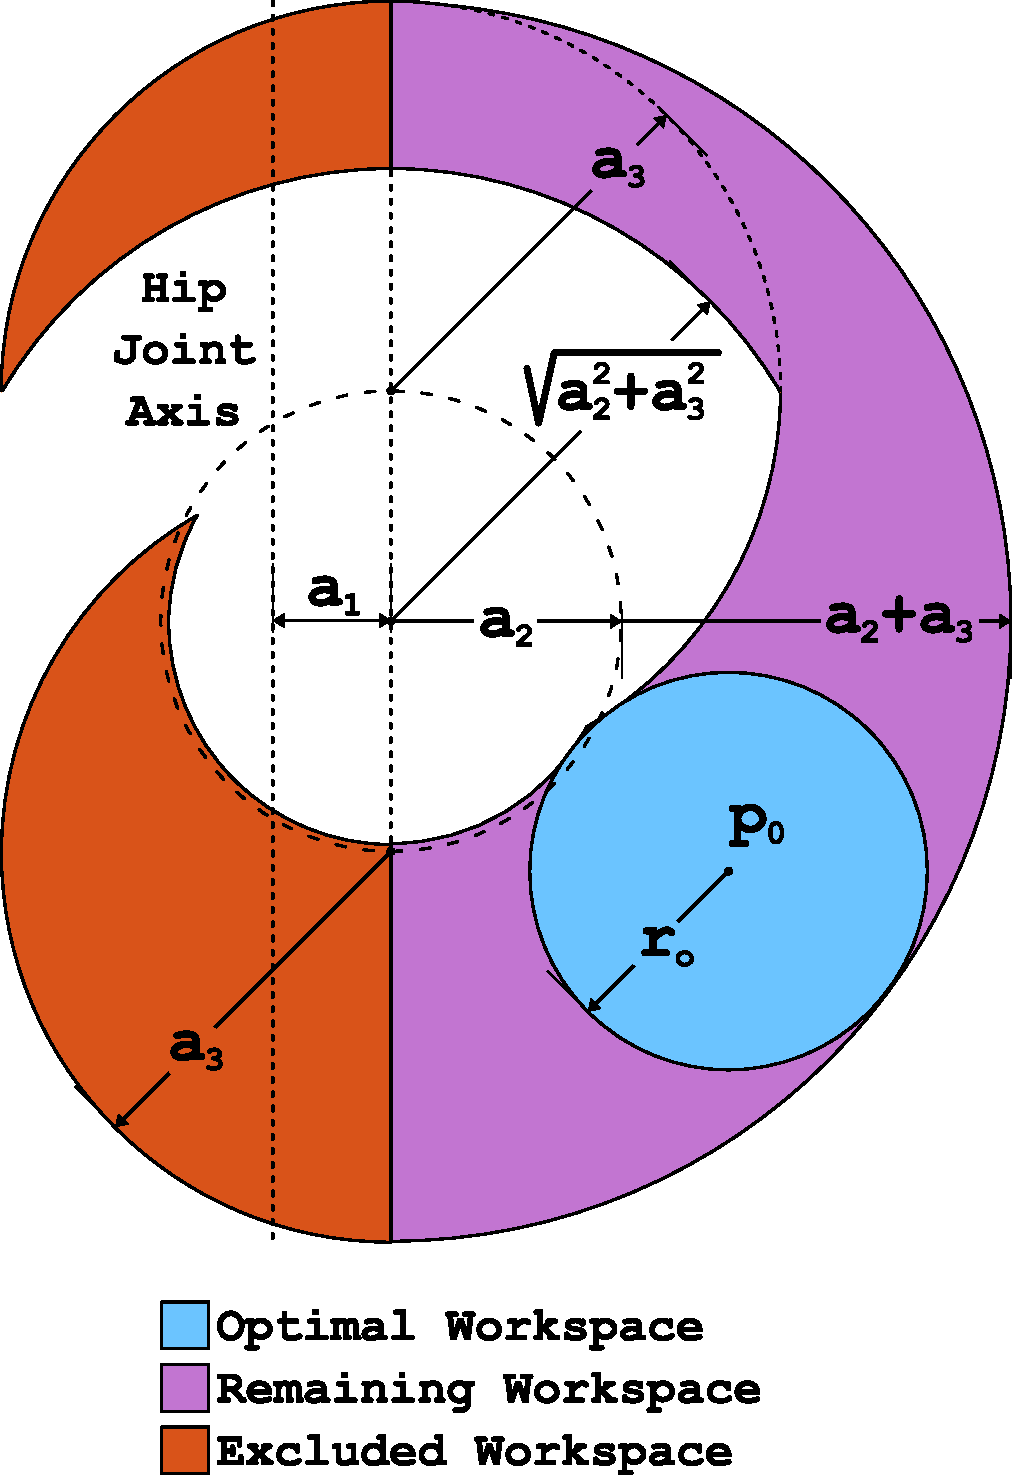
\includegraphics[width=0.7\textwidth]{images/workspace.pdf}
    \caption{Reachable Workspace Section for $q_1 = 0$}
    \label{fig:workspace_analysis}
\end{figure}

The actuator limits are the primary constraints defining this space. These limits are imposed both by the
physical components (i.e. the finite rotational range of the servo-motors) and by the mechanical design itself,
which is configured to prevent self-collision between links and other limbs.
For this specific implementation, the joint constraints are defined as follows:
\begin{equation*}
  q =[q_1, q_2, q_3]^T \in
  \left[-30^\circ, 30^\circ \right]
  \times
  \left[-90^\circ, 90^\circ \right]
  \times
  \left[30^\circ, 180^\circ \right]
\end{equation*}

As an additional safety measure, a portion of the resulting workspace (the red coloured area in Figure
\ref{fig:workspace_analysis}) is excluded from operation to prevent collisions with the robot's body or the mounting
structure. A simplified and safe \textbf{Optimal Work Region} is then defined by inscribing a sphere within the
remaining viable workspace depicted in blue. The center of this sphere, $p_0$, is designated as the leg's nominal
\textbf{Rest Position}, which will serve as the origin for gait trajectories.


\subsection{Trajectory Design}

Moving to trajectory generation, the goal is to create a function $p_d$ to define the motion of the foot.
The design of this trajectory is guided by several key principles and assumptions. Firstly, the path
must be parametric, dependent on both the desired walking speed $v$ and the direction of movement $\psi$.
Secondly, the trajectory primitive is generated relative to the leg's central rest position $p_0$, which is
eventually added as a final offset to determine the absolute path $p_d(t)$. For this initial derivation, we
also assume the ground is a flat, predictable plane at a constant height set to 0 (or $p_{z,0}$ after applying
the rest offset).

The gait cycle is composed of two distinct and well defined phases, which needs to be properly stitched together
to ensure smooth ($C^2$) motion. During the \textbf{Stance Phase}, the foot must remain stationary relative to
the ground as the body moves forward. This implies that the foot's velocity relative to the robot's body must
be constant and equal to $-v$ (along the $\psi$ direction). Consequently, the acceleration during this linear
phase is zero. Conversly, during the \textbf{Swing Phase}, the leg should relocate to start a new cycle
while also lifting off the ground.


\subsubsection{Quintic Polynomials}

The simplest and most widely adopted solution in robotics is using fifth-order (quintic) polynomials
\cite{biagiotti2008trajectory, siciliano2009robotics} to move between two points while matching boundary
conditions for position, velocity, and acceleration. A generic quintic polynomial is defined by six
coefficients ($c_0, \dots, c_5$):

$$ p(t) = c_5t^5 + c_4t^4 + c_3t^3 + c_2t^2 + c_1t + c_0 $$

The function $p(t)$ represents the position, while its first and second time derivatives, $v(t)$ and $a(t)$,
represent the velocity and acceleration, respectively:

$$ v(t) = \frac{dp}{dt} = 5c_5t^4 + 4c_4t^3 + 3c_3t^2 + 2c_2t + c_1 $$
$$ a(t) = \frac{d^2p}{dt^2} = 20c_5t^3 + 12c_4t^2 + 6c_3t + 2c_2 $$

To solve for the six unknown coefficients $\mathbf{c} = [c_0, c_1, c_2, c_3, c_4, c_5]^T$, we impose six
known boundary conditions, i.e. the desired position, velocity, and acceleration at the start time ($t = 0$)
and at the end time ($t = T$), where $T$ is the total duration of the movement. Then a system of six linear
equations can be derived and expressed in matrix form as $M \cdot \mathbf{c} = \mathbf{b}$:

$$
  \begin{bmatrix}
    1 & 0 & 0 & 0 & 0 & 0 \\
    0 & 1 & 0 & 0 & 0 & 0 \\
    0 & 0 & 2 & 0 & 0 & 0 \\
    1 & T & T^2 & T^3 & T^4 & T^5 \\
    0 & 1 & 2T & 3T^2 & 4T^3 & 5T^4 \\
    0 & 0 & 2 & 6T & 12T^2 & 20T^3
  \end{bmatrix}
  \begin{bmatrix}
    c_0 \\ c_1 \\ c_2 \\ c_3 \\ c_4 \\ c_5
  \end{bmatrix}
  =
  \begin{bmatrix}
    p_0 \\
    v_0 \\
    a_0 \\
    p_f \\
    v_f \\
    a_f
  \end{bmatrix}
$$

The vector of coefficients $\mathbf{c}$ can then be found by inverting the $6 \times 6$ matrix $M$ and
multiplying it by the vector of boundary conditions $\mathbf{b}$:

\begin{equation}
  \mathbf{c} = M^{-1} \cdot \mathbf{b}
  \label{eqn:quintic_poly_solution}
\end{equation}

The resulting coefficients are constants that depend only on the specified boundary conditions and the total
movement time $T$. The final trajectory $p(t)$ is then a continuous function of the generic time variable
$t \in [0, T]$.


\subsubsection{Horizontal Component}

We start by defining the 1D horizontal component of the trajectory, $p_h(t)$, as a function of normalized time
$t \in [0, 1]$, and representing the motion along the direction of travel $\psi$. The 2D path in the $XY$ plane
is simply this 1D motion projected onto the direction vector $\mathbf{d}(\psi) = [\sin(\psi), \cos(\psi)]^T$.

We define the \textbf{Duty Factor} $\beta$ as the fraction of the cycle spent in the Stance Phase (typically
$\beta > 0.5$ for structural stability, meaning that the robot is supported by at least 3 contact points at every
moment). This divides the normalized unit period into two segments:

$$ T_{stance} = \beta $$
$$ T_{swing} = (1-\beta) $$

The cycle is thus defined with the Swing Phase occurring for $t \in [0, T_{swing}]$ and the Stance Phase for
$t \in [T_{swing}, 1]$. The trajectory oscillates between a forward limit (touchdown) $p_1 = r$ and a backward
limit (liftoff) $p_2 = -r$. The total horizontal stroke is $S = 2r$.

During the Stance Phase, the motion is linear, connecting the touchdown point (at $t = T_{swing}$, $p = r$) to
the liftoff point (at $t = 1$, $p = -r$). The function $p_{h,stance}(t)$ is the equation of this line. Its slope,
the normalized velocity $v_{norm}$ is constant:

$$ v_{norm} = \frac{\Delta p}{\Delta t} = \frac{-2r}{\beta} $$
The trajectory for this phase and its derivatives are given by:
$$ p_{h,stance}(t) = p_1 + v_{norm} \cdot (t - T_{swing}) $$
$$ v_{h,stance}(t) = v_{norm} $$
$$ a_{h,stance}(t) = 0 $$
During the Swing Phase, we use the quintic polynomial method to move from the liftoff position back to the
touchdown position. This function must smoothly connect the end of the previous stance phase (at $t = 1$,
or $t = 0$ in the new cycle) to the start of the current stance phase (at $t = T_{swing}$).

To ensure $C^2$ continuity, we must match the position, velocity, and acceleration of the stance phase at both
ends. We solve for the polynomial $p_{h,swing}(t)$ over the interval $T = T_{swing}$ using the following
boundary conditions vector $\mathbf{b}_{h,swing} = [-r, v_{norm}, 0, r, v_{norm}, 0]^T$.
Solving Equation \ref{eqn:quintic_poly_solution} with this vector yields the specific coefficients for the
horizontal swing polynomial.


\subsubsection{Vertical Component}

Next, we define the vertical component of the motion, $p_z(t)$, relative to the ground plane.

During the stance phase the foot is on the ground providing propulsion, therefore $p_{z,stance}(t) = 0$. This
implies $v_{z,stance} = 0$ and $a_{z,stance}(t) = 0$.

During the swing phase, the leg must lift to a clearance height $H_{lift}$ ($= r$) and return to the ground.
This motion must also be $C^2$ continuous, connecting smoothly to the zero-motion of the Stance Phase. To
achieve this, the Swing Phase is split into two identical halves, "Lift-Up" and "Lift-Down", each with duration
$T_{lift} = T_{swing} / 2$.

We solve for the lift-up polynomial $p_{z,up}(t)$. The boundary conditions must match the stance phase at the
start ($t = 0$) and ensure a smooth apex at the peak ($t = T_{lift}$). The boundary conditions vector is
$\mathbf{b}_{z,up} = [0, 0, 0, H_{lift}, 0, 0]^T$. Then, the lift-down polynomial is a time-mirrored version of
the lift-up segment.

This two-stage approach guarantees $C^2$ continuity for the entire vertical trajectory: it starts from
$p=0, v=0, a=0$ (matching the stance end), achieves a smooth peak at $t = T_{lift}$, and returns to
$p=0, v=0, a=0$ at $t = T_{swing}$ (matching the stance start).


\subsubsection{Path Assembly}

The complete spatial geometry of the gait, $p_{prime}(t)$ is now fully designed, as a function of the
normalized time $t \in [0, 1]$. The complete primitive is assembled by combining the horizontal and vertical
components, projecting the horizontal motion onto the $X$ and $Y$ axes, and stitching the swing and stance
phases together:
$$
p_{prime}(t) =
  \begin{cases}
    \begin{bmatrix}
      p_{h,swing}(t) \sin(\psi) \\
      p_{h,swing}(t) \cos(\psi) \\
      p_{z,swing}(t)
    \end{bmatrix}
    & \text{Swing: } 0 \le t < T_{swing} \\
    \\
    \begin{bmatrix}
      p_{h,stance}(t) \sin(\psi) \\
      p_{h,stance}(t) \cos(\psi) \\
      0
    \end{bmatrix}
    & \text{Stance: } T_{swing} \le t \le 1 \\
  \end{cases}
$$
The desired path $p_d(t)$ sent to the controller is then obtained by biasing this primitive with the
leg's central rest position $p_d(t) = p_0 + p_{prime}(t)$.

Crucially, this formulation decouples the path's spatial geometry from its execution speed.
The function $p_{prime}(t)$ defines only the geometric path, with the input $t$ representing the percentage
of cycle completion, not the actual time.


\subsubsection{Walking Speed Dependance}

The desired physical walking speed $v$ is introduced by controlling how fast this normalized time $t$ advances
in the real world. This is achieved through a discrete-time implementation. First, we determine the required
real-time period ($T_{real}$) for one full gait cycle. The physical stroke $S = 2r$ must be covered at the
desired velocity $v$ during the stance phase, which lasts for a fraction $\beta$ of the total period, therefore
the total real-time period for the cycle is:
$$ T_{real} = \frac{2r}{\beta v} $$
In the control loop, the normalized path $p_{prime}(t)$ is discretized into $n$ samples (e.g. $n = 1000$).
A counter $k$ (where $0 \le k < n$) tracks the current step, and the corresponding normalized time is $t_k = k/n$.
The controller achieves the desired velocity $v$ by incrementing the counter $k$ at a specific real-time
frequency, $f$ determined by the real-time step $\Delta t_{real}$, which is the total period divided by the
number of samples:
$$ \Delta t_{real} = \frac{T_{real}}{n} = \frac{2r}{n \beta v} $$
The controller's update frequency is $f = 1 / \Delta t_{real}$. By adjusting this frequency $f$ (or its inverse,
the time step $\Delta t_{real}$), the desired velocity $v$ is precisely controlled, while the spatial trajectory
remains constant.
\section{Control and Simulation}
\label{sc:simulation}

Having defined the complete kinematic model via the DH parameters, derived the IK solver, and designed a $C^2$
continuous gait trajectory, we proceed to validate the entire system by simulation. To verify that these
theoretical components function correctly in unison, a digital model of the leg is implemented in the
Simulink \cite{matlab} environment. This simulation serves as a crucial proof-of-concept, allowing for the
verification of the control logic and the workspace before committing to physical hardware. This section details
the open-loop control architecture used for this validation and the construction of the simulation model itself.


\subsection{Open Loop Control Strategy}

The control strategy adopts an open-loop architecture (Figure \ref{fig:control_chain}), deliberately neglecting
external disturbances or modeling errors; its sole purpose is to validate the correctness of the kinematic chain.

It consists in:

\begin{itemize}
  \item \textbf{Path Planning:} The Gait Trajectory Generator outputs the desired Cartesian position $p_d(t)$
    at each time step, given a desired walking speed $v$ and direction $\psi$.
  \item \textbf{Inverse Kinematics:} The desired path $p_d(t)$ is fed into the IK solver, which
    calculates the required vector of joint angles $q_d(t) = [q_1, q_2, q_3]^T$ needed to achieve
    that end-effector position.
  \item \textbf{Leg Model (Plant):} The desired angles $q_d(t)$ are sent as commands to the
    digital twin of the leg, modeled with the aid of the Simscape library.
  \item \textbf{Forward Kinematics:} For validation, the actual joint angles from the simulation model are
    fed into the FK block (based on the DH Table \ref{tab:dh_parameters}). This calculates the resulting
    end-effector position, $p_{sim}(t)$.
\end{itemize}

\begin{figure}[htbp]
    \centering
    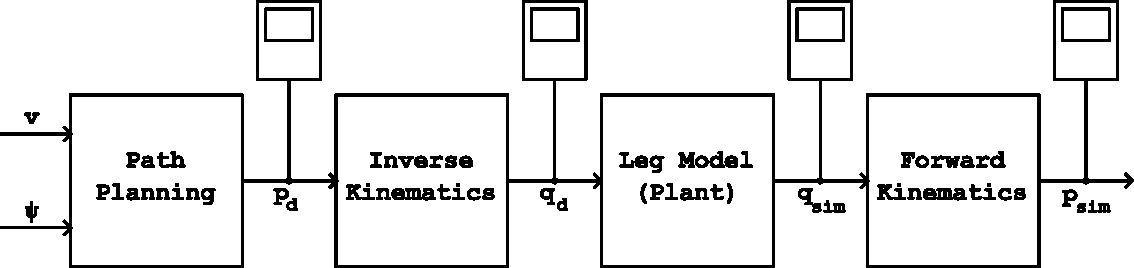
\includegraphics[width=0.98\textwidth]{images/open_loop.pdf}
    \caption{Block Diagram of the Open Loop Control Chain.}
    \label{fig:control_chain}
\end{figure}

A key assumption at this stage is the use of ideal actuators. The joints in the simulation are modeled as
ideal position controllers. This means that when a joint is commanded to go to an angle $q_i$, it achieves
this setpoint almost instantaneously and without error. We are intentionally neglecting the dynamics of the
motors (e.g. torque limits, friction, PID control, and settling time) to isolate the validation purely to the
kinematic model.

The goal is to answer the question: "If the joints go to the angles we calculated, does the foot go to the
position we intended?" The simulation is considered successful if the error between the desired path and the
actual path is approximately close to zero for the entire duration.


\subsection{Digital Simulation}

To create a realistic and physically-grounded representation of the leg, the digital twin is constructed using
Simscape Multibody \cite{simscape}. This MATLAB/Simulink toolbox allows for the modeling of 3D mechanical systems
by defining rigid bodies, joints, constraints, and their spatial relationships.

The leg model (reported in Figure \ref{fig:simscape_model}) is built by importing the CAD (Computer-Aided Design)
files for each link (Coxa, Femur, and Tibia) for a better graphical representation. These rigid bodies are then
connected using 'Revolute Joint' and 'Transformation' blocks at the appropriate locations, corresponding to the
physical actuators and established DH parameters. The joint axes and link-to-link coordinate frames are meticulously
aligned ensuring the simulation model is a one-to-one representation of the theoretical kinematic chain.

\begin{figure}[htbp]
    \centering
    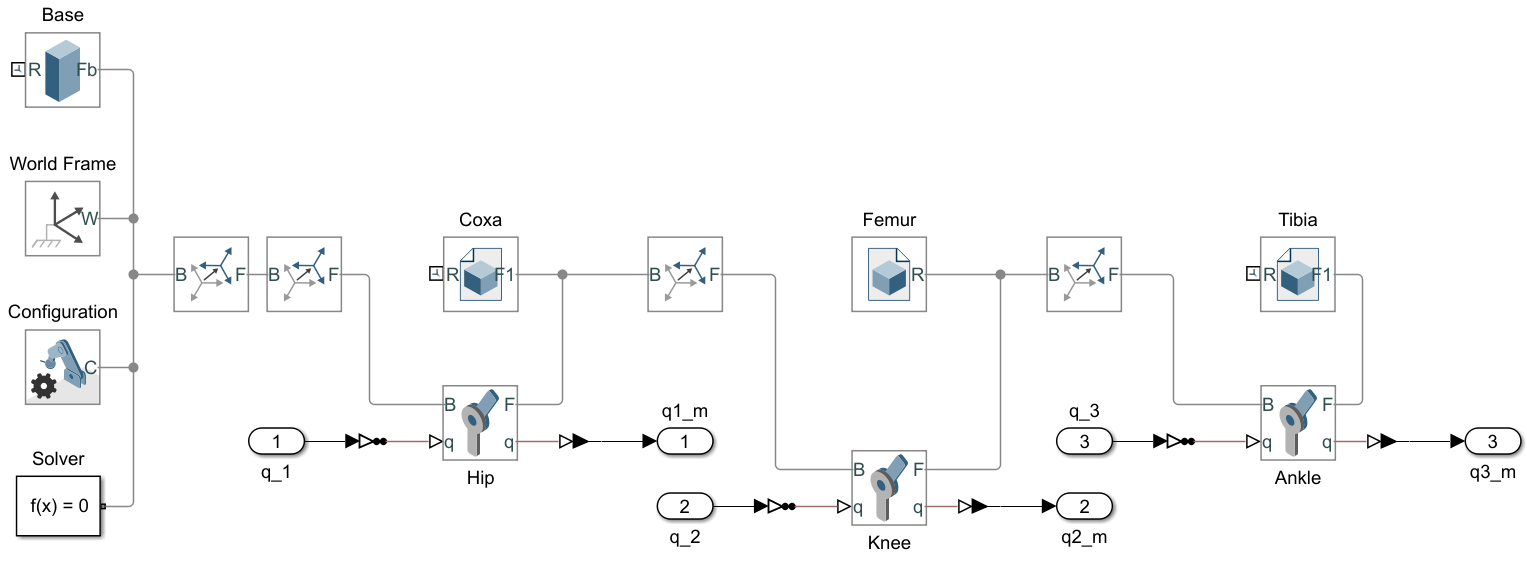
\includegraphics[width=0.98\textwidth]{images/simscape.PNG}
    \caption{Simscape Multibody Limb Model (Plant Block).}
    \label{fig:simscape_model}
\end{figure}

This model serves as the 'Plant' block in the control diagram. The inputs to the model are the three desired
joint angles $q_d(t)$ from the IK block, which drive the 'Sensing and Motion' input of the Revolute
Joint blocks. The outputs are the resulting joint angles and poses, which are passed to the FK validation block
and used to generate the 3D animation (as seen in Figure \ref{fig:rendering_side}) for visual confirmation
of the gait.

\begin{figure}[htbp]
    \centering
    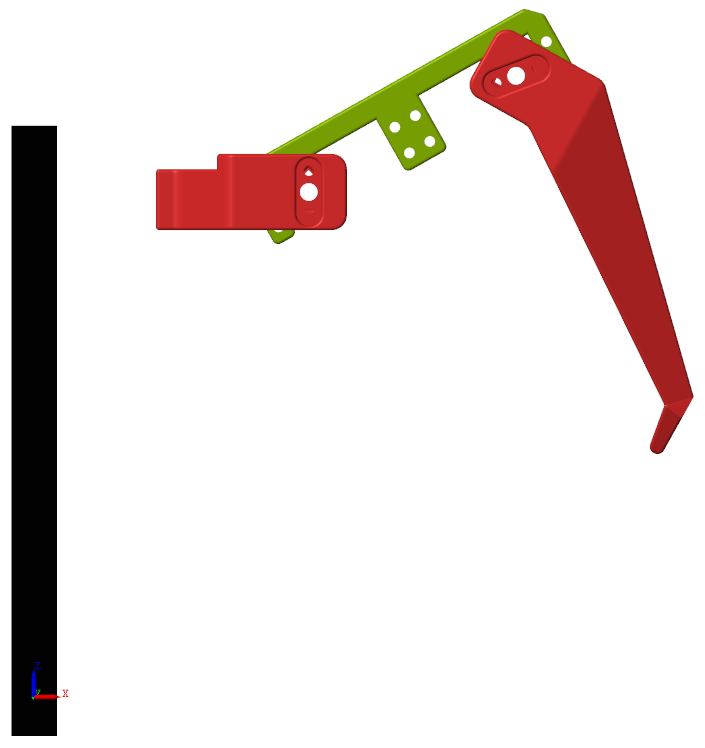
\includegraphics[width=0.48\textwidth]{images/model_side.PNG}
    \caption{3D Rendering of the Simscape Simulation (Side View).}
    \label{fig:rendering_side}
\end{figure}

For the purpose of the digital simulation, the walking direction will be set to be coincident with the y axis
($\vec{\psi} = \vec{y}$).


\subsection{Simulation Results}
\label{sec:simulation_results}

The primary validation of the theoretical model comes from a comparison of the desired Cartesian path (the output
of the Path Generator, $p_d$) against the actual path achieved by the Simscape model (the output of the Forward
Kinematics block, $p_{sim}$). These two trajectories (Figure \ref{fig:gait_z_psi}) are undistinguishable,
confirming the entire kinematic chain — from the DH parameters and IK solver to the FK validation — is
mathematically correct and consistent.

\begin{figure}[htbp]
    \centering
    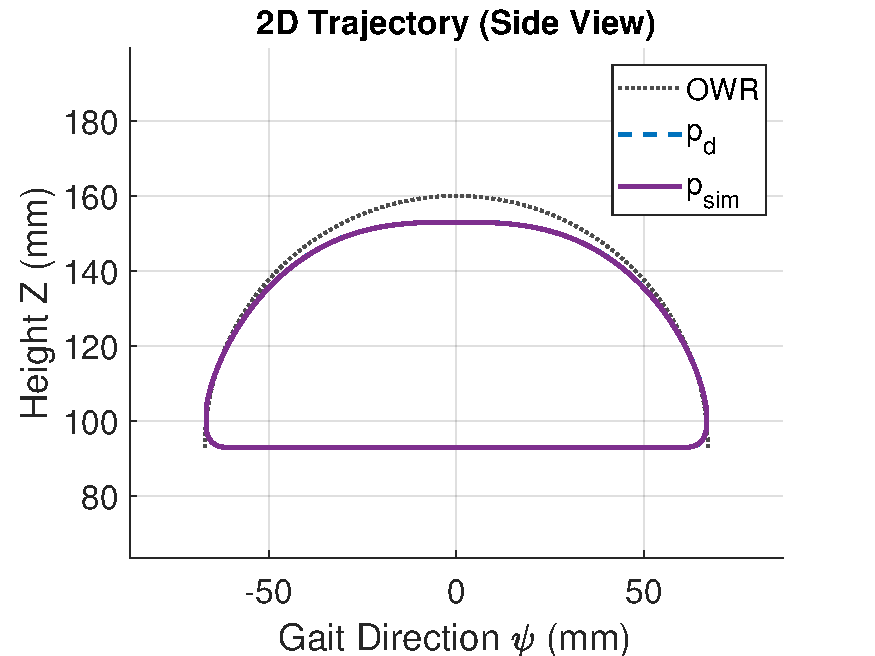
\includegraphics[width=0.65\textwidth]{images/gait_z_psi.pdf}
    \caption{Simulated Gait Ttrajectory in the $Z\psi$-plane (Side View).}
    \label{fig:gait_z_psi}
\end{figure}

The path clearly shows the linear stance phase (where Z is constant) and the smooth, $C^2$ continuous swing
phase, which lifts the foot to the required clearance height. Furthermore, the entire trajectory operates
correctly within the boundaries of the predefined Optimal Workspace Region (OWR).


\subsubsection{Cartesian Space Analysis}

A comprehensive overview of the system's performance in Cartesian space is depicted in Figure \ref{fig:cartesian_results}.

The three plots (X, Y, Z) demonstrate a perfect tracking of the commanded trajectory ($p_d$) as expected from the
ideal actuator assumption. The negligible errors ($e_{sim} \le 0.8\,mm$) are attributed to inertial effects
and a small tracking delay, both reasonable assumptions in real world systems.

\begin{figure}[htbp]
    \centering
    \begin{subfigure}[b]{0.8\textwidth}
        \centering
        
\includegraphics[width=\textwidth]{images/cartesian_trajectories.pdf}
        \caption{Trajectory Tracking}
    \end{subfigure}

    \begin{subfigure}[b]{0.8\textwidth}
        \centering
        
\includegraphics[width=\textwidth]{images/cartesian_errors.pdf}
        \caption{Tracking Errors}
    \end{subfigure}
    \caption{Cartesian-Space Simulation Results.}
    \label{fig:cartesian_results}
\end{figure}


\subsubsection{Joint Space Analysis}

Figure \ref{fig:joint_results} confirms that the Cartesian trajectory is correctly translated into smooth,
continuous joint commands, free of any "snaps" or sudden changes even at phase transition points.

Furthermore, all three trajectories operate comfortably within the designated joint limits, confirming the IK
solver is capable of finding a valid and safe solution.

\begin{figure}[htbp]
    \centering
    \begin{subfigure}[b]{0.8\textwidth}
        \centering
        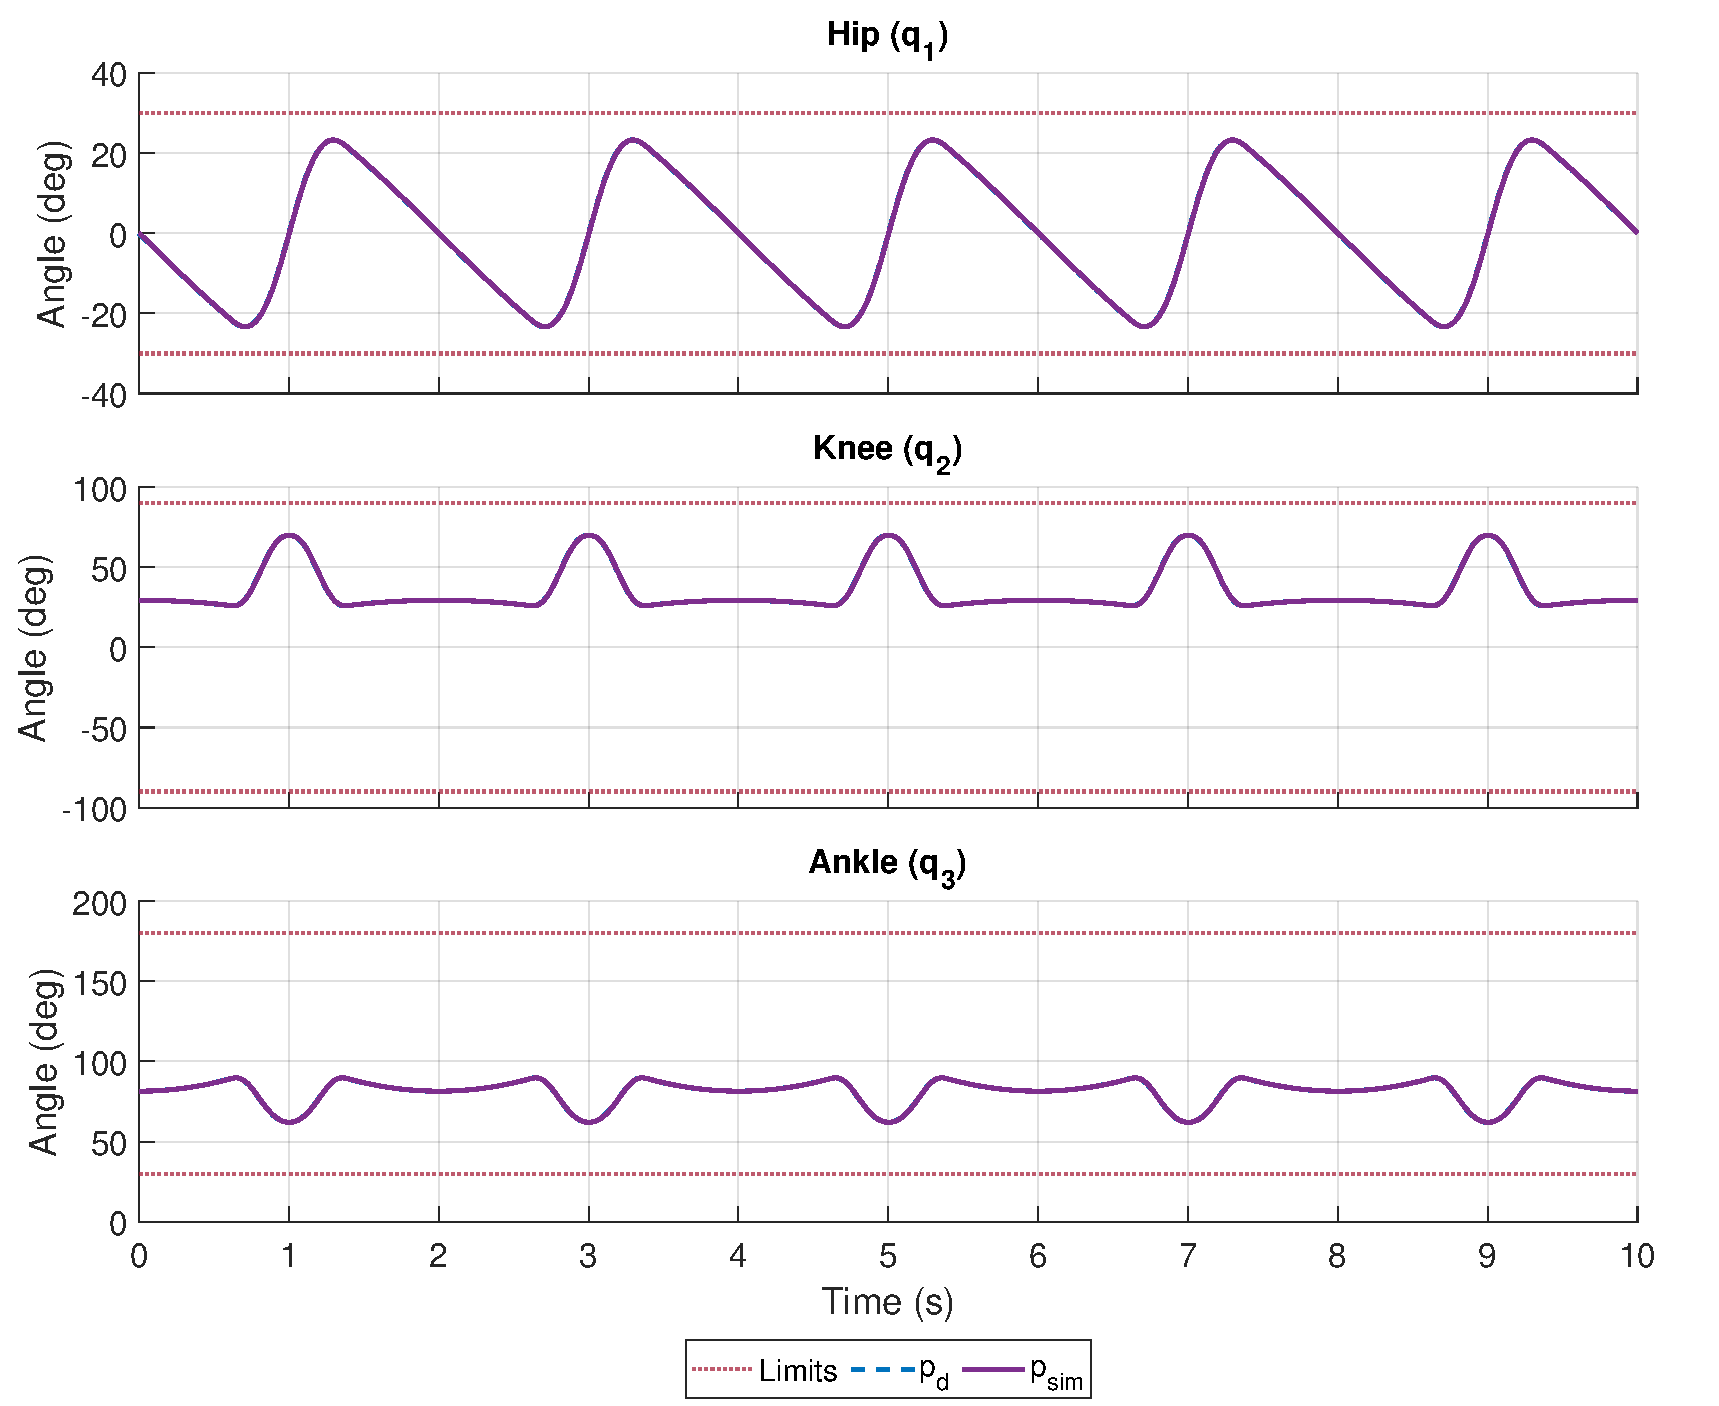
\includegraphics[width=\textwidth]{images/joint_trajectories.pdf}
        \caption{Trajectory Tracking}
    \end{subfigure}

    \begin{subfigure}[b]{0.8\textwidth}
        \centering
        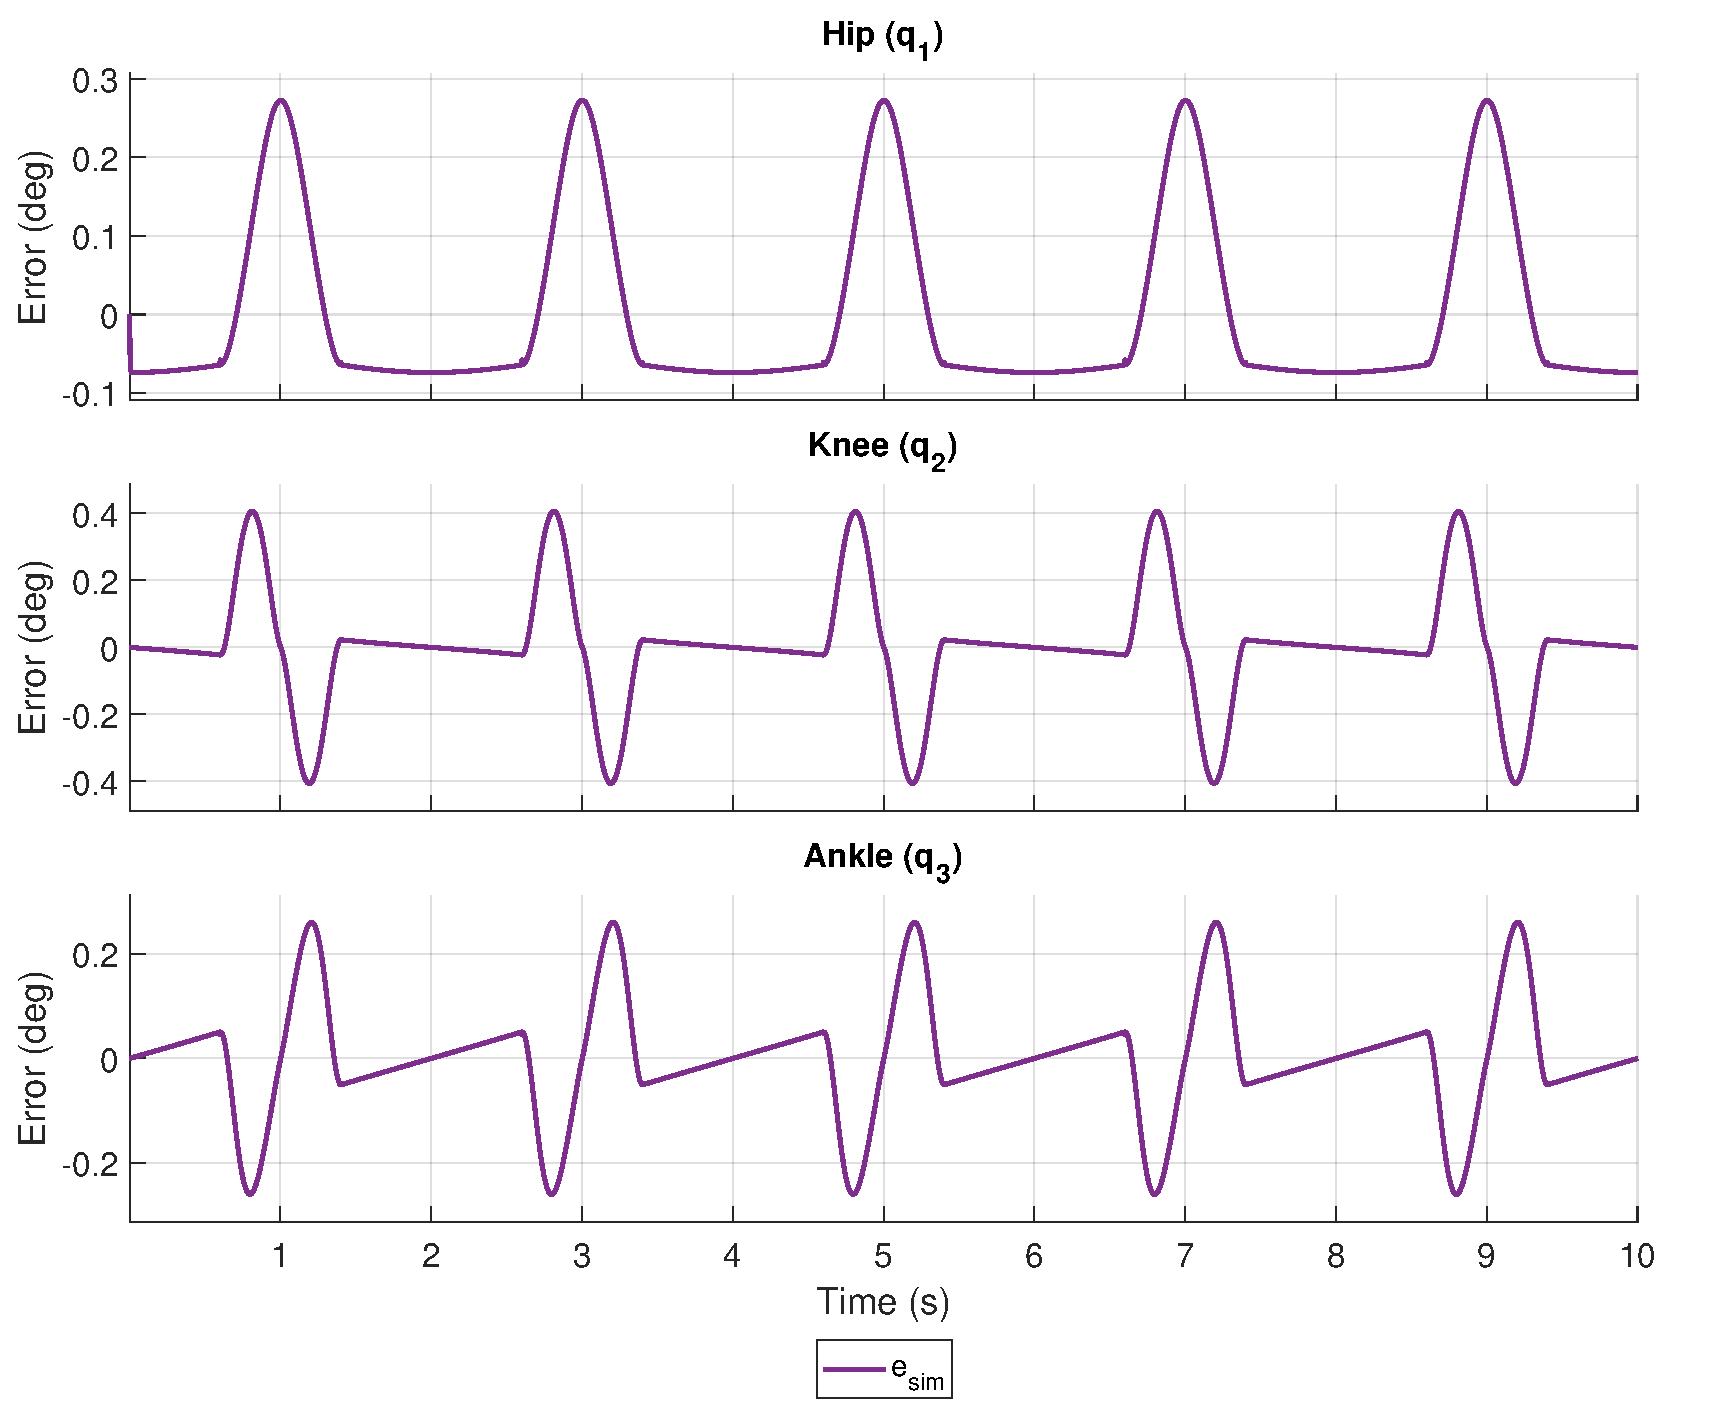
\includegraphics[width=\textwidth]{images/joint_errors.pdf}
        \caption{Tracking Errors}
    \end{subfigure}
    \caption{Joint-Space Simulation Results.}
    \label{fig:joint_results}
\end{figure}

\section{Proprioception and Path Adaptation}
\label{sec:proprioception}

The open-loop control strategy and kinematic chain validated in Section 2.2 demonstrated the system's theoretical
correctness under ideal conditions. However, this approach relies on the strict assumption of a perfectly flat
and predictable terrain ($z_{ground} = p_{z,0}$). In a real-world unstructured environment, ground elevation
varies unpredictably. Without feedback, a purely time-driven limb would either strike the ground prematurely
— causing high mechanical stress and potential instability — or fail to reach it entirely, compromising propulsion.

To relax this assumption and enable a "Blind Walking" \cite{brooks1989robot} capability, the system is
augmented with basic proprioceptive sensing and a reactive control layer. Admittedly, while this approach does
not fully solve the locomotion problem for extreme terrain (which would require a more structured control), it
represents the fundamental first step towards robust locomotion: the ability to detect and adapt to the ground
surface upon contact.


\subsection{Contact Sensing and Architectural Shift}

To detect the ground transition, the limb is equipped with a binary contact sensor located at the tip of the
foot. This sensor acts as a logical limit switch, providing a boolean signal $S_c$ to the controller:

$$
  S_c =
  \begin{cases}
    1 & \text{if touching ground}\\
    0 & \text{otherwise}
  \end{cases}
$$

The introduction of this sensor demands a fundamental shift in the control architecture. The path planning
problem transforms from a purely time-dependent function, $p_d(t)$, to a state-dependent system driven by
discrete events.

In the previous open-loop model, the gait phase was dictated by a global clock. In this adaptive model, the
controller must monitor $S_c$ and be capable of interrupting the Swing Phase exactly at the moment of
physical impact. Consequently, the trajectory generator cannot simply map a normalized time $t \in [0,1]$ to a
position; it must be restructured to handle asynchronous events and variable phase durations.


\subsection{Finite State Trajectory Generator}

To implement this reactive logic robustly, a custom Finite State Machine (FSM, Figure \ref{fig:fsm_logic}) was designed
\cite{cruse1990mechanisms}. This generator decouples the logical phase of the leg from the global clock,
allowing for local adaptations while maintaining synchronization through a phase-advance mechanism.

\begin{figure}[htbp]
    \centering
    \begin{tikzpicture}[
        ->,                       % Freccia su tutti i percorsi
        >=Stealth,                % Stile punta freccia moderno
        node distance=3.5cm and 4.5cm, % Distanza verticale e orizzontale
        every state/.style={      % Stile globale per i cerchi degli stati
            draw=black,
            thick,
            fill=gray!10,
            minimum size=3cm,     % Dimensione fissa per cerchi uniformi
            align=center          % Permette "a capo" dentro i cerchi
        },
        thick                     % Linee spesse
    ]

    % --- Definizione degli Stati ---

    % 1. Stance 1 (Alto-Sinistra) - Stato Iniziale
    \node[state, initial left, initial text={Start}] (S1) {Posterior\\Stance\\(Stance 1)};

    % 2. Lift (Alto-Destra) - A destra di S1
    \node[state] (Lift) [right=of S1] {Lift\\(Early Swing)};

    % 3. Touch (Basso-Destra) - Sotto a Lift
    \node[state] (Touch) [below=of Lift] {Touch\\(Late Swing)};

    % 4. Stance 2 (Basso-Sinistra) - A sinistra di Touch (e sotto S1)
    \node[state] (S2) [left=of Touch] {Anterior\\Stance\\(Stance 2)};

    % --- Transizioni (Frecce) ---

    % 1. Stance 1 -> Lift (Freccia verso destra)
    \path (S1) edge node[above, align=center] {
        $p_h \le -r$
    } (Lift);

    % 2. Lift -> Touch (Freccia verso il basso)
    \path (Lift) edge node[right, align=left] {
        $t > T_{lift}$
    } (Touch);

    % 3. Touch -> Stance 2 (Freccia verso sinistra)
    \path (Touch) edge node[below, align=center] {
        $S_c = 1$ \\
        \textit{-- or --} \\
        $t > T_{swing}$
    } (S2);

    % 4. Stance 2 -> Stance 1 (Freccia verso l'alto)
    \path (S2) edge node[left, align=right] {
        $p_h = 0$
    } (S1);

    \end{tikzpicture}
    \caption{Finite State Machine for Adaptive Trajectory Generation.}
    \label{fig:fsm_logic}
\end{figure}


\subsubsection{State 1: Posterior Stance (Stance 1)}

The initial state of the cycle. Geometrically, it corresponds to the leg moving from the central rest
position ($p_h = 0$) towards the posterior limit of the workspace ($p_h = -r$).

\newpage
The horizontal velocity is constant ($\dot{p}_h = -v$). The position is calculated via a discrete-time
integrator, which is reset upon entering the state. The vertical position $z$ is held constant at the
previously detected ground level.

Upon entering this state, the system calculates a synchronization parameter, $\delta(k)$, to compensate for any
timing drift accumulated in the previous cycle $k-1$. Recalling the duty factor $\beta$, the parameter is calculated as:
\begin{equation}
  \delta(k) = \left(1 - \frac{\beta}{2}\right) - t - \delta(k-1)
\end{equation}
where $t$ is the normalized global time counter. This ensures that the leg remains synchronized with the
robot's gait rhythm, correcting for local timing variations.

The system transitions to the Lift state when the horizontal position reaches the posterior stroke limit
($p_h \le -r$).


\subsubsection{State 2: Lift Phase (Early Swing)}

This state represents the deterministic part of the swing phase, where the leg lifts off the ground to clear
potential obstacles.

The duration of this phase, $T_{lift}$, is dynamically calculated to absorb the phase error $\delta(k)$:
\begin{equation}
  T_{lift} = T_{touch} + \delta(k) = \frac{1-\beta}{2} + \delta(k)
\end{equation}
This variable duration is the mechanism that re-synchronizes the leg with the robot's global gait cycle.

A quintic polynomial moves the foot vertically from its current height to the clearance height $H_{lift}$ over
the duration $T_{lift}$, while another quintic polynomial starts repositioning the foot horizontally over the
duration $T_{swing} = T_{lift} + T_{touch}$.

The state transitions only when the timer exceeds the allocated time ($t > T_{lift}$), meaning the foot has
reached the desired clearence height.


\subsubsection{State 3: Touch Phase (Late Swing)}

This state governs the descent of the leg. Crucially, this is where proprioceptive feedback is expected to trigger.

The timer variable is adjusted to parametrize the descent polynomial $t' = t_{norm} - T_{lift}$, guiding the
foot from $H_{lift}$ back towards the nominal ground ($z = 0$) over a fixed duration $T_{touch} = (1-\beta)/2$.
The global timer is maintained to preserve continuity with the swing phase dynamics.

The system exits this state under two distinct conditions:

\begin{enumerate}
  \item \textbf{Time-out:} The time expires ($t' > T_{touch}$ or equivalently $t > T_{swing}$), implying the leg
    completed the full trajectory without contact (e.g. a hole or flat ground).
  \item \textbf{Early Contact:} The sensor triggers ($S_c = 1$). This indicates the ground is higher
    than expected (e.g. an obstacle).
\end{enumerate}

In both cases, the FSM immediately transitions to the next state.


\subsubsection{State 4: Anterior Stance (Stance 2)}

Following the touchdown, the leg enters the anterior portion of the stance phase, moving from the anterior limit
($+r$ or the early contact point) back towards the central rest position ($p_h = 0$).

The horizontal velocity returns to $-v$. The vertical position $z$ is locked at the specific height recorded at
the moment of the Touch $\to$ Anterior Stance transition. This allows the robot to walk "on top" of obstacles rather
than trying to push through them.

The cycle completes when the leg crosses the zero-point of the workspace ($p_h = 0$), triggering the transition
back to Posterior Stance. At this crossing, the cycle index $k$ increments, and the loop repeats.


\subsection{Adaptive Simulation Results}

To validate the proprioceptive controller, the Simscape environment was modified to include an uneven terrain
profile.

Figure \ref{fig:adaptive_results} provides a direct comparison between the nominal, time-based trajectory
and the reactive, adaptive trajectory generated by the FSM in the presence of uneven terrain. For visual
clarity, these plots represent the trajectory primitives defined in the $Z\psi$-plane.


\subsubsection{Vertical Adaptation}

The bottom plot (Vertical Trajectory) clearly demonstrates the effectiveness of the proprioceptive loop. When
the limb encounters a positive obstacle (represented by the gray terrain profile), the adaptive trajectory
deviates from the nominal path exactly at the moment of impact. Unlike the nominal reference, which would
attempt to drive the foot through the terrain, the adaptive system triggers an immediate transition from the Touch
Phase to the Stance Phase. The vertical position is subsequently maintained at the obstacle's height for the
duration of the propulsion stroke, effectively allowing the robot to walk on top of the irregularity rather than
pushing against it.

\begin{figure}[htbp]
    \centering
    
\includegraphics[width=0.98\textwidth]{images/adaptive_comparison.pdf}
    \caption{Adaptive Gait Simulation with the New FSM Trajectory Generator.}
    \label{fig:adaptive_results}
\end{figure}


\subsubsection{Synchronization and Phase Correction}

Despite the timing disturbances introduced by early ground contacts, the top plot (Horizontal Trajectory) shows
that the system maintains robust synchronization. While the early impact inevitably causes a minor phase lead
(visible as a slight horizontal shift between the purple and green waves), the trajectory does not drift
indefinitely. Instead, when the obstacle is no longer present, the cycle realigns with the non-adaptive ideal
trajectory. This proves that the phase synchronization mechanism successfully compensates for these delays in
subsequent cycles, keeping the limb's rhythm bounded and consistent with the global gait cycle.


\subsubsection{Continuity and Stability Considerations}

There is key consideration to address regarding the kinematic continuity at the impact point: while the
generated trajectory primitives are designed to be $C^2$ continuous, the very nature of the "Blind Walk"
implies that the exact moment of touchdown is unpredictable. Consequently, when the ground is struck earlier
than planned, the vertical velocity changes abruptly from the descent speed to zero (relative to the terrain).
Therefore, at these specific transition points, strict $C^2$ continuity cannot be guaranteed.

Secondly, while effective as a proof of concept, this adaptive generator has specific limitations. For starters,
it currently compensates only for elevated obstacles (protrusions), neglecting potential depressions or holes
in the terrain. Also, unlike the nominal generator, this reactive strategy does not inherently guarantee that
the modified path remains within the Optimal Workspace Region (OWR); without explicit saturation limits, the
adaptation could potentially request kinematically unfeasible positions.

Another important consideration to keep in mind is the dynamic shortening of the foot's contact time introduces
significant stability challenges; therefore, a rigorous balance study is essential for the future implementation
of the full robot.

In summary, this strategy is designed specifically to handle minor terrain irregularities (roughness) rather
than large obstacles, representing a solid foundation for higher level obstacle avoidance planning and control
\cite{saranli2001rhex}.
    \chapter{Custom Smart Actuator Module Design}
\label{ch:servomotor}

The performance of any articulated robotic system is strictly bound by the capabilities of its actuators.
In the context of the hexapod limb designed in Chapter \ref{ch:model}, the requirements for
trajectory tracking accuracy, and smoothness of motion are strict. While the geometric design dictates
the reachable workspace, the actuator dynamic dictates the quality of movement within that space.

To satisfy these requirements without incurring in the prohibitive costs of industrial-grade servomotors
(e.g. Dynamixel-X series \cite{robotis_dynamixel_x}), a custom actuator module was developed, aiming for a good
compromise between performance and cost. This section details the transition from analyzing the limitations of
standard low-cost components to the engineering of a high-performance, "smart" joint module.

\section{Limitations of Commercial Servos}
\label{sec:limitations}

The initial prototyping phase considered the use of the MG996R \cite{mg996r}, a ubiquitous standard-size
servomotor widely adopted in hobbyist robotics. However, a rigorous characterization revealed fundamental
limitations that rendered these units unsuitable for high-fidelity gait control.

The critical deficiencies, ranked by their impact on system performance, are:

\begin{itemize}
    \item \textbf{Feedback Sensor Degradation:} The internal feedback mechanism relies on a low-cost
        resistive potentiometer. Unlike non-contact solutions, this component involves a physical wiper
        sliding over a resistive track. Continuous operation leads to mechanical wear, causing progressive
        signal degradation and non-linearity. This deterioration was experimentally identified as the
        primary source of long-term positioning error.

    \item \textbf{Deadband and Stick-Slip Behavior:} To prevent motor hunting, the MG996R specifies a dead
        band width of $5\,\mu s$~\cite{mg996r}. When combined with the high static friction (stiction) of
        the metal gear assembly, this results in a significant effective dead-zone, making the joint fail
        to move for small command increments.

    \item \textbf{Limited Control Resolution and Bandwidth:} The standard PWM control protocol is inherently
        limited by the update rate. As per specifications, the MG996R operates on a $20\,ms$ period ($50\,Hz$
        frequency)~\cite{mg996r}. This low update frequency acts as a bottleneck for high-dynamic control loops,
        introducing a delay of up to $20\,ms$ between command and actuation.

    \item \textbf{Manufacturing Variability:} Significant unit-to-unit inconsistency was observed regarding
        the operational range characteristics. Two identical servos receiving the same PWM signal often
        align to different physical angles. This lack of repeatability makes the IK model unreliable without
        an intensive, individual calibration for each joint.

    \item \textbf{Obsolete Open-Loop Architecture:} Finally, as confirmed by the standard 3-pin interface
        (PWM, $V_{cc}$, GND)~\cite{mg996r}, these servos operate as "black boxes". The internal PID
        controller is hard-wired and inaccessible, preventing the implementation of advanced friction
        compensation or different control architectures in general. Crucially, the lack of feedback (current,
        real position, temperature) prevents any form of centralized Hardware-in-the-Loop control or online
        diagnostics.
\end{itemize}

To visualize and confirm the newly introduced limitations, an experimental characterization was performed
on two randomly selected units (Motor A and Motor B). The results, presented in Figure
\ref{fig:servo_deficiencies}, map the control signal pulse width ($T_{on}$) against the actual output
angle measured by a high-precision external magnetic encoder. The test involved a full sweep from $0.5\,ms$
to $2.5\,ms$ (Forward path, blue line) followed by a return to $0.5\,ms$ (Backward path, orange line).

\begin{figure}[htbp]
    \centering
    \begin{subfigure}[b]{0.48\textwidth}
        \centering
        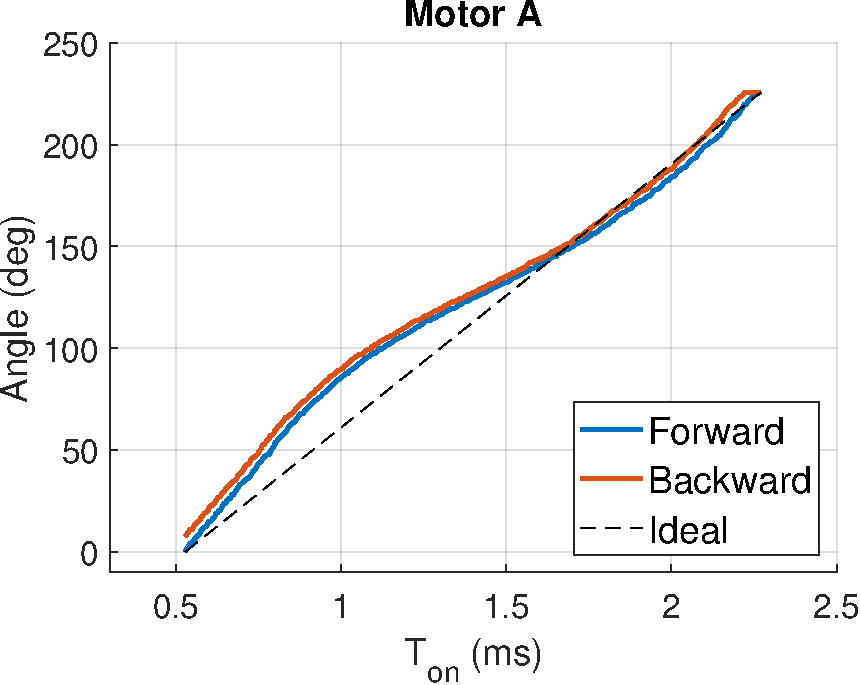
\includegraphics[width=\textwidth]{images/motor_char_A.pdf}
        \caption{}
        \label{fig:motor_A}
    \end{subfigure}
    \hfill
    \begin{subfigure}[b]{0.48\textwidth}
        \centering
        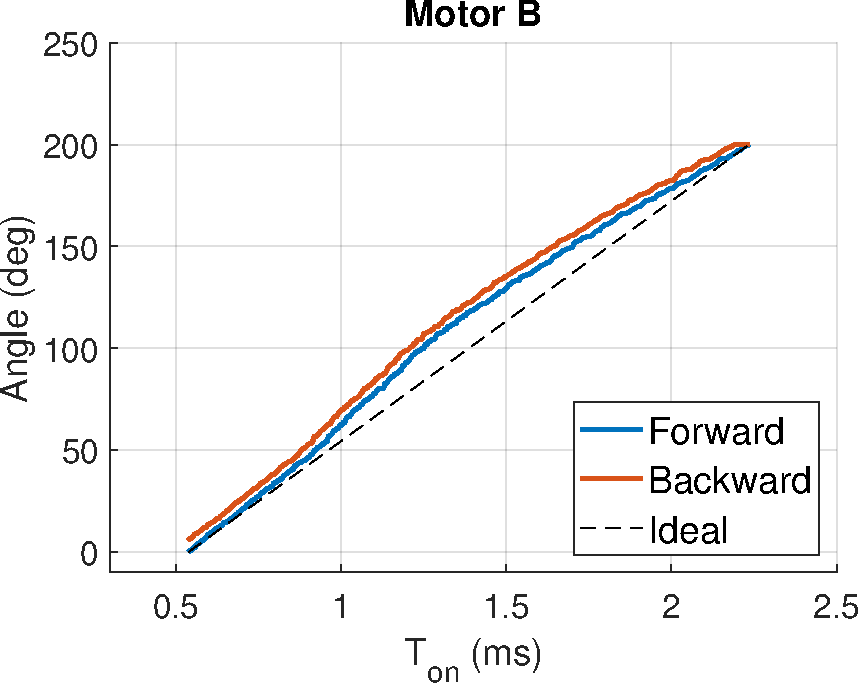
\includegraphics[width=\textwidth]{images/motor_char_B.pdf}
        \caption{}
        \label{fig:motor_B}
    \end{subfigure}
    \caption{Experimental Characterization of two MG996R Units.}
    \label{fig:servo_deficiencies}
\end{figure}

The dashed black line represents the ideal linear response ($Angle \propto T_{on}$) expected from a servomotor,
adjusted for the motor effective operative range. Both units show severe deviations from this ideal behavior,
introducing position errors exceeding $15^{\circ}$ thus making precise open-loop control impossible without a
complex, motor-specific calibration lookup table.

Furthermore, both plots exhibit a considerable hysteresis loop, visible as the vertical gap between the
forward and backward trajectories for the same PWM input.

Perhaps the most critical finding is the discrepancy between the two nominally identical units. Motor A covers
a range of approximately $0^{\circ}$ to $230^{\circ}$, while Motor B, driven by the exact same signal, spans a
smaller range from roughly $0^{\circ}$ to $200^{\circ}$. It should be noted that the graphs have been truncated
at the endpoints where a change in $T_{on}$ failed to produce any change in output position, indicating
mechanical or electronic saturation.

This inconsistencies confirms that a unified kinematic model cannot be applied to a robot using these actuators.
Each joint would require individual characterization and compensation, which is impractical for scalable
deployment.

Finally, although not visible at this macro-scale zoom, the stepped nature of the data acquisition
(confirmed during testing) revealed that the motors often remained stationary for input changes of
$5-10\,\mu s$ (corresponding to $1-2$ PWM step increments @$50\, Hz$), jumping only when the accumulated
error overcame the internal deadband and static friction.

Given these fundamental constraints, simply upgrading to a slightly more expensive hobby servo would yield
diminishing returns. The only viable solution was to redesign the control electronics entirely, retaining only
the mechanical shell and the DC motor, to create a fully programmable, closed-loop actuator.

\section{Hardware Design and Component Selection}
\label{sec:hardware}

The design of the custom actuator module is driven by a set of strict functional and physical requirements
derived from the limitations identified in the previous section.

The most critical requirement is maintaining the exact external form factor of the original servo. This
allows for a "drop-in replacement" into the existing hexapod limb structure without mechanical modification.
Consequently, all control electronics must be miniaturized to fit within the original motor chassis volume
(approx. $40 \times 20 \times 36$ mm).

The steady-state positioning error should ideally be reduced to $<\pm 0.5^{\circ}$ to enable precise
point-to-point gait control and the control interface could shift from a time-based PWM signal to a digital bus
protocol, enabling bi-directional communication (telemetry) and flexible control, while also simplifying
scalability.


\subsubsection{Position Feedback: Magnetic Encoder (AS5600)}

To eliminate the degradation issues of resistive potentiometers, the ams AS5600 \cite{as5600} magnetic rotary
position sensor was selected. This contactless sensor measures the orientation of a diametric magnet mounted
directly on the output shaft. Key advantages include:

\begin{itemize}
    \item \textbf{Contactless Operation:} Eliminates friction and mechanical wear, significantly extending
        the operational lifespan.
    \item \textbf{High Precision:} The sensor provides a 12-bit resolution over a full rotation,
        corresponding to a theoretical precision of $0.088^{\circ}$ per step ($360^{\circ}/4096$), which is
        well above the $0.5^{\circ}$ requirement.
    \item \textbf{Digital Interface:} It communicates via a robust $\text{I}^2\text{C}$ bus, reducing the
        susceptibility to electromagnetic noise inherent in analog ADC lines within the motor housing.
\end{itemize}


\subsubsection{Power Stage: H-Bridge Driver (DRV8870)}

To drive the DC motor, the DRV8870 \cite{drv8870} was chosen for its straightforward interface and integrated
protection features. Unlike the discrete transistor bridges often found in cheap servos, this integrated
H-bridge supports up to $3.6\,\text{A}$ peak current, comfortably handling the motor's stall current. The
driver allows for:

\begin{itemize}
    \item \textbf{Bi-directional Control:} Full forward/reverse driving via logic-level inputs and internal
        shoot-through protection, automatically handling the dead-time to prevent short circuits across the
        power rails during direction changes.
    \item \textbf{PWM Speed Control:} Compatible with high-frequency switching to reduce audible noise.
    \item \textbf{Integrated Protection:} Automatic current regulation (chopping) and thermal shutdown,
        protecting the electronics from stall conditions common in legged locomotion.
\end{itemize}


\subsubsection{Control Logic: Microcontroller (STM32F103C8T6)}

The "brain" of the module is the STM32F103C8T6 \cite{stm32f103c8t6}, a 32-bit ARM Cortex-M3 microcontroller.
This component was selected for its superior computational power ($72\,\text{MHz}$), necessary to execute the
real-time control algorithms, and for its comprehensive development ecosystem.

The key peripherals are the two $I^2C$ buses used for internal and external communication and interface:

\begin{itemize}
    \item \textbf{Internal Bus:} Dedicated high-speed channel for reading the AS5600 position sensor and
        interfacing with potential future on-board peripherals (e.g. EEPROM or current sensing).
    \item \textbf{External Bus:} The main interface for the actuator module. This will allows multiple
    servos to be daisy-chained on a single bus, eliminating the need for external PWM expansion boards (e.g.
    PCA9685) and simplifying the robot's wiring harness.
\end{itemize}

Additionally, the timer/PWM peripheral will accurately control the driver module.


\subsection{PCB Design and Layout}

All selected components, along with necessary passive elements (bypass capacitors, pull-up resistors, etc...),
were integrated into a custom-designed Printed Circuit Board (PCB). To respect the strict volume constraint,
the board was designed with specific dimensions to replace the original control board inside the servo case.
Additionally, an exposed 5-pin header provides access to the SWD interface (Serial Wire Debug), allowing for
firmware flashing and real-time debugging.

Detailed schematics of the board are provided in Appendix \ref{app:pcb} while the completed design can be seen
in Figures \ref{fig:pcb_layout} and \ref{fig:motor_result}. Note that provision was made for additional future
peripheral (e.g. current sensing), although outside the scope of the current experimental validation.

\begin{figure}[htbp]
    \centering
    \begin{subfigure}[b]{0.18\textwidth}
        \centering
        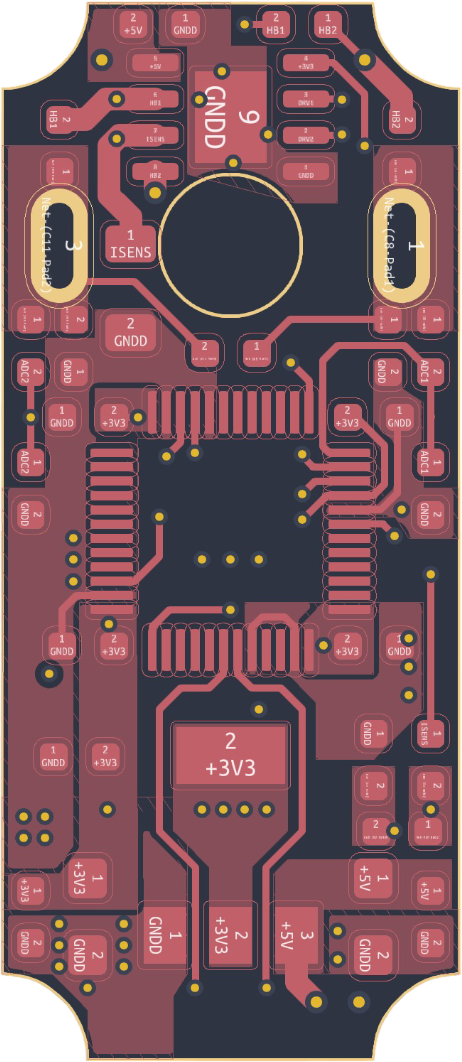
\includegraphics[width=\textwidth]{images/front_cad_pcb.png}
        \caption{CAD Front}
    \end{subfigure}
    \hfill
    \begin{subfigure}[b]{0.18\textwidth}
        \centering
        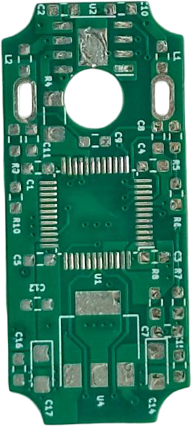
\includegraphics[width=\textwidth]{images/front_real_pcb.png}
        \caption{Real Front}
    \end{subfigure}
    \hfill
    \begin{subfigure}[b]{0.18\textwidth}
        \centering
        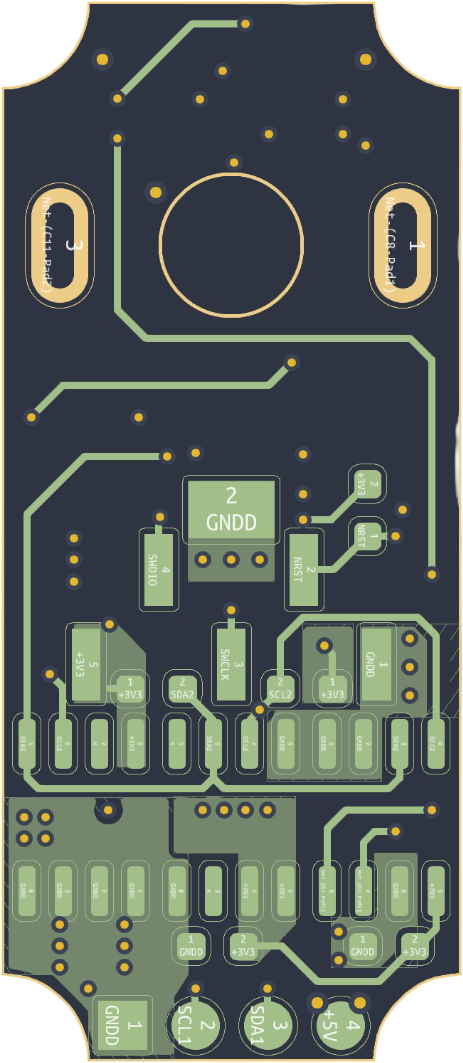
\includegraphics[width=\textwidth]{images/bottom_cad_pcb.png}
        \caption{CAD Bottom}
    \end{subfigure}
    \hfill
    \begin{subfigure}[b]{0.18\textwidth}
        \centering
        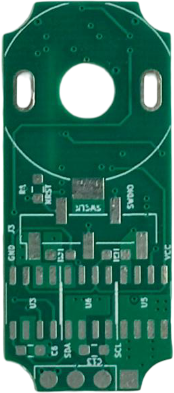
\includegraphics[width=\textwidth]{images/bottom_real_pcb.png}
        \caption{Real Bottom}
    \end{subfigure}
    \caption{Custom PCB Layout Design (CAD and Real).}
    \label{fig:pcb_layout}
\end{figure}

\begin{figure}[htbp]
    \centering
    \begin{subfigure}[b]{0.98\textwidth}
        \centering
        
\includegraphics[width=\textwidth]{images/front_motor.png}
        \caption{Front Side}
    \end{subfigure}

    \begin{subfigure}[b]{0.98\textwidth}
        \centering
        
\includegraphics[width=\textwidth]{images/bottom_motor.png}
        \caption{Bottom Side}
    \end{subfigure}
    \caption{Populated Custom PCB, i.e. Smart Actuator Internals.}
    \label{fig:motor_result}
\end{figure}
\section{Embedded Software Architecture}

The firmware running on the STM32 microcontroller was developed using a modular, object-oriented approach in
C++. This architecture ensures code reusability, encapsulation of hardware specifics, and ease of maintenance
and scalability. The software stack (Appendix \ref{app:software}) is organized into four distinct abstraction
layers, moving from low-level hardware management to high-level application logic.


\subsubsection{Layer 1: Vendor HAL}

The foundational layer consists of the Hardware Abstraction Layer (HAL) provided by the microcontroller
manufacturer. Modules such as \texttt{i2c.h} and \texttt{tim.h} handle the direct register-level configuration
of the MCU peripherals. Relying on these standard verified drivers ensures robust handling of interrupts and
basic I/O operations.


\subsubsection{Layer 2: Custom Middleware and Communication}

This layer acts as a bridge between the raw hardware and the high-level logic, abstracting the communication
protocols. Key modules include:

\begin{itemize}
    \item \textbf{I2C Device Wrappers:} Classes like \texttt{i2c\_device} and \texttt{i2c\_slave} extend the
        Vendor HAL to provide simplified interfaces for bus communication, handling read/write buffers and
        addressing logic.
    \item \textbf{Virtual Register:} This is the core component of the communication architecture. It
        implements the "Virtual Register Map" concept, abstracting the internal state of the actuator
        (positions, gains, modes) as a set of memory-mapped values. This allows the external master to
        interact with the servo seamlessly, as if reading from a standard memory device, changing its
        behaviour dynamically as needed.
\end{itemize}


\subsubsection{Layer 3: High-Level Component Drivers}

This layer contains the specific drivers for the chosen hardware components and the pure algorithmic logic,
independent of the specific MCU.

\begin{itemize}
    \item \textbf{Component Drivers:} The \texttt{AS5600} and \texttt{DRV8870} classes encapsulate the
        specific operational details of the sensor and driver. They utilize the lower layers to perform tasks
        such as reading raw magnetic angles or setting PWM duty cycles, exposing clean methods (e.g.
        \texttt{getAngle()}, \texttt{setSpeed()}) to the application layer.
    \item \textbf{Math and Control:} This module contains the implementation of the control algorithms,
        including the Switching PID logic. It is designed to be purely mathematical, accepting error inputs
        and producing control outputs without direct dependencies on hardware headers.
\end{itemize}


\subsubsection{Layer 4: Application Layer}

The highest level of the hierarchy integrates all previous modules to define the actuator's behavior.

\begin{itemize}
    \item \textbf{Smart Servo Class:} This main class encapsulates the entire logic of the actuator. It
        instantiates the drivers and control modules, managing the data flow between the sensor readings,
        the PID computation, and the motor output.
    \item \textbf{Entry Point:} The \texttt{main.cpp} and \texttt{CONFIG.h} files handle the system
        initialization, configuration, and the execution of the main real-time control loop.
\end{itemize}


\subsection{Control Strategy}

Achieving high-precision positioning in robotic joints is inherently challenging due to the presence of
nonlinear friction phenomena \cite{armstrong1994survey}, specifically static friction (Coulomb) and velocity
weakening effects (Stribeck). As extensively discussed in control literature, standard linear controllers like
the classical PID struggle to manage these non-linearities effectively.

In particular, the integral action required to overcome static friction often leads to overshoot. When
combined with the Stribeck effect, this energy imbalance prevents convergence to the setpoint, resulting in
persistent oscillations known as the "hunting phenomenon". While model-based control techniques could
theoretically compensate for these effects, they require precise parameter identification — which is difficult
to maintain over time due to wear and load changes — and impose a computational burden often incompatible with
low-cost embedded hardware.

A robust alternative that seems to mitigate these issues without requiring complex friction models is the
class of hybrid control strategies, such as Reset or Switching PID \cite{bisoffi2020stick, lorigiola2025switching}.
These approaches modify the internal state of the controller (specifically the integrator) based on discrete
logical rules triggered by the system's state (e.g. zero-crossing of the error or velocity).

The control strategy implemented in this custom actuator is directly derived from the Switching PID strategy
proposed and analyzed in \cite{lorigiola2025switching}. This approach uses a state-machine logic to
dynamically switch the integrator behavior and avoid hunting.

Since the rigorous mathematical derivation and stability proofs of this control strategy are extensive and already
well-documented in the referenced literature, they are considered outside the scope of this thesis. Instead,
this section provides a functional description of the algorithm and the pseudocode implementation specifically
tailored for the custom hardware application.


\subsubsection{Algorithm Description}

\begin{algorithm}[H]
    \footnotesize
    \caption{Switching PID for Friction Compensation}
    \label{alg:switching_pid}
    \begin{algorithmic}[1]
        \Require Reference $r_k$, Measurement $y_k$, Gains $K_p, K_i, K_d$
        \Ensure Control Input $u_k \in [-1, 1]$

        \State $e_k \gets r_k - y_k$ \Comment{Position Error}
        \State $v_k \gets \frac{y_k - y_{k-1}}{\Delta t}$ \Comment{Estimated Velocity}

        \vspace{0.1cm}

        % --- BLOCCO 1: PI Computation (Blu) ---
        \ColorBlock{RoyalBlue}{
            \textbf{1. PI Computation \& Anti-Windup} \\
            $\sigma \gets K_i \cdot e_k$ \\
            $\phi' \gets K_p \cdot (e_k + I_{state})$ \\
            $\phi \gets \text{Saturation of }\phi'$ \\
            $\Delta_{sat} \gets \phi' - \phi$ \\
            \textbf{if} $\text{sgn}(\sigma) == \text{sgn}(\Delta_{sat})$ \textbf{and} $\Delta_{sat} \ne 0$ \textbf{then} \\
            \hspace*{1.5em} $I_{state} \gets I_{state}$ \Comment{Hold integrator} \\
            \textbf{else} \\
            \hspace*{1.5em} $I_{state} \gets I_{state} + \sigma \Delta t$ \Comment{Update integrator} \\
            \textbf{end if}
        }

        \vspace{0.1cm}

        % --- BLOCCO 2: Switching Logic (Arancione) ---
        \ColorBlock{OrangeRed}{
            \textbf{2. Switching Logic} \\
            \textbf{if} $(\text{State} == \textsc{StickSlip}) \textbf{ and } (\sigma \cdot \phi \le 0)$ \textbf{then} \\
            \hspace*{1.5em} $\phi \gets -\phi$ \Comment{Reset energy} \\
            \hspace*{1.5em} $I_{state} \gets \frac{\phi}{K_p} - e_k$ \\
            \hspace*{1.5em} $\text{State} \gets \textsc{Overshoot}$ \\
            \textbf{else if} $(\text{State} == \textsc{Overshoot}) \textbf{ and } (v_k \cdot \phi \ge 0)$ \textbf{then} \\
            \hspace*{1.5em} $\phi \gets K_p \cdot \sigma / K_i$ \Comment{Restore linear behavior} \\
            \hspace*{1.5em} $I_{state} \gets 0$ \\
            \hspace*{1.5em} $\text{State} \gets \textsc{StickSlip}$ \\
            \textbf{end if}
        }

        \vspace{0.1cm}

        % --- BLOCCO 3: Output (Verde) ---
        \ColorBlock{ForestGreen}{
            \textbf{3. Output Calculation} \\
            $u_k \gets \text{Clamp}(\phi - K_d \cdot v_k, -1, 1)$
        }

        \vspace{0.1cm}

        \State \Return $u_k$
    \end{algorithmic}
\end{algorithm}

The control loop runs at a fixed frequency of $1\,\text{kHz}$. At each time step $k$, the algorithm described
in Algorithm \ref{alg:switching_pid} is executed.

The controller operates in two distinct logical states: when in \textbf{Stick-Slip State} (default) the
integrator is fully active to build up the torque necessary to overcome static friction ($F_s$). The logic
prioritizes "breaking out" of the stick phase. Detecting that the error has crossed zero (overshoot) triggers
the transition to the \textbf{Overshoot State}. In this mode, the logic serves to dampen the response by
inverting the control action, preventing the limit cycles (hunting) typical of high-gain PIDs on frictional loads.

The transition between these states is governed by the relationship between the generalized position error
($\sigma$) and the total proportional-integral control effort ($\phi$).

Notably, the term $\phi$ acts as a 'virtual' control effort that is reset discontinuously during state
transitions (Block 2), allowing the controller to instantly adapt its energy based on the
friction regime, a capability not present in standard linear PIDs.

This control strategy is originally derived for set-point regulation (point-to-point motion). While effective for
the quasi-static segments of the gait cycle, its application to dynamic trajectory tracking may require further
tuning or structural modifications (e.g. feed-forward terms). Addressing these specific dynamic tracking
optimization is considered outside the scope of this thesis and is left for future work.




\section{Module Characterization and Benchmarking}

The mechanical design and control strategy were validated by subjecting the custom actuator module to an
experimental characterization mirroring the one applied to to the commercial units in Section
\ref{sec:limitations} The tests were conducted using the integrated AS5600 magnetic sensor for feedback,
with the module powered at a nominal voltage of $6.7\,\text{V}$. The $\text{I}^2\text{C}$ bus was used to
transmit the target position directly as a 12-bit digital setpoint, bypassing the resolution limits of
standard PWM signaling.


\subsection{Static Analysis: Linearity and Hysteresis}

The first validation step focused on the static input-output relationship. A slow triangular ramp reference
($100\,ms$ per sensor LSB) spanning the full range in both Forward and Backward directions was administered
to the module. Figure \ref{fig:custom_linearity} illustrates the experimental results.

Compared to the commercial servo baseline (refer to Figure \ref{fig:servo_deficiencies}), the custom module
demonstrates significant visible improvements:

\begin{itemize}
    \item \textbf{Linearity:} The response closely follows the ideal characteristic $y=x$. The distortion,
        typical of the potentiometer-based commercial unit, is effectively eliminated.
    \item \textbf{Hysteresis Suppression:} The forward and backward paths are virtually indistinguishable at
        full scale. The removal of the mechanical potentiometer in favor of the non-contact magnetic sensor
        drastically reduces mechanical backlash, ensuring high repeatability regardless of the direction of
        approach.
    \item \textbf{Range Extension:} The operating range is no longer constrained by the physical limits of
        the potentiometer, granting access to the full $360^\circ$ of rotation. This continuous capability
        necessitates software phase unwrapping to ensure seamless transitions across the zero-crossing point.
\end{itemize}

\begin{figure}[htbp]
    \centering
    \begin{subfigure}[c]{0.48\textwidth}
        \centering
        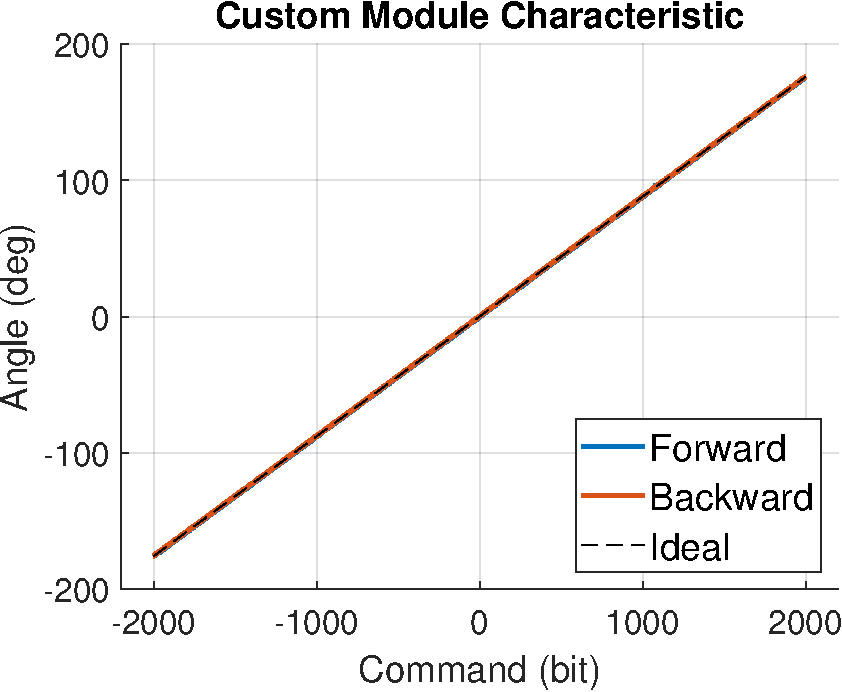
\includegraphics[width=\textwidth]{images/custom_linearity.pdf}
        \caption{Full-scale linearity analysis.}
        \label{fig:custom_linearity_full}
    \end{subfigure}
    \hfill
    \begin{subfigure}[c]{0.48\textwidth}
        \centering
        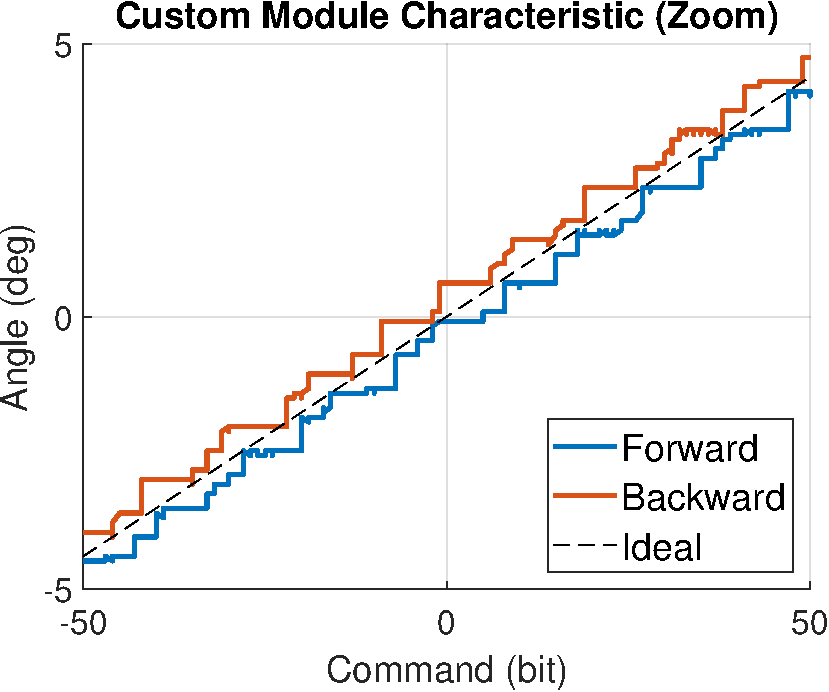
\includegraphics[width=\textwidth]{images/custom_linearity_zoom.pdf}
        \caption{Zoomed view showing micro-linearity.}
        \label{fig:custom_linearity_zoom}
    \end{subfigure}
    \caption{Input-Output Characteristic of the Custom Actuator.}
    \label{fig:custom_linearity}
\end{figure}


\subsection{Step Response Analysis: Sensitivity and Settling}

The module was then subjected to a series of step commands (square waves) of varying amplitudes: Micro-step
($1^\circ$), Mid-range ($15^\circ$), and Full-scale ($90^\circ$).

The results, presented in Figure \ref{fig:step_responses} and \ref{fig:step_error}, highlight two key behaviors:

\begin{itemize}
    \item \textbf{Resolution and Sensitivity ($1^\circ$):} Unlike the commercial unit, which exhibited a
        significant deadband preventing fine adjustments, the custom module responds reliably to micro-step
        commands as small as $1^\circ$ ($\approx 11$ LSB). Note that the visible jitter at this stage is sensor
        noise.
    \item \textbf{Transient Response ($15^\circ, 90^\circ$):} For larger transitions, the motor reaches the
        target setpoint rapidly. While a slight overshoot is visible, the system settles quickly without
        entering a limit cycle (hunting), validating the effectiveness of the Switching PID control algorithm.
\end{itemize}

\begin{figure}[htbp]
\centering
    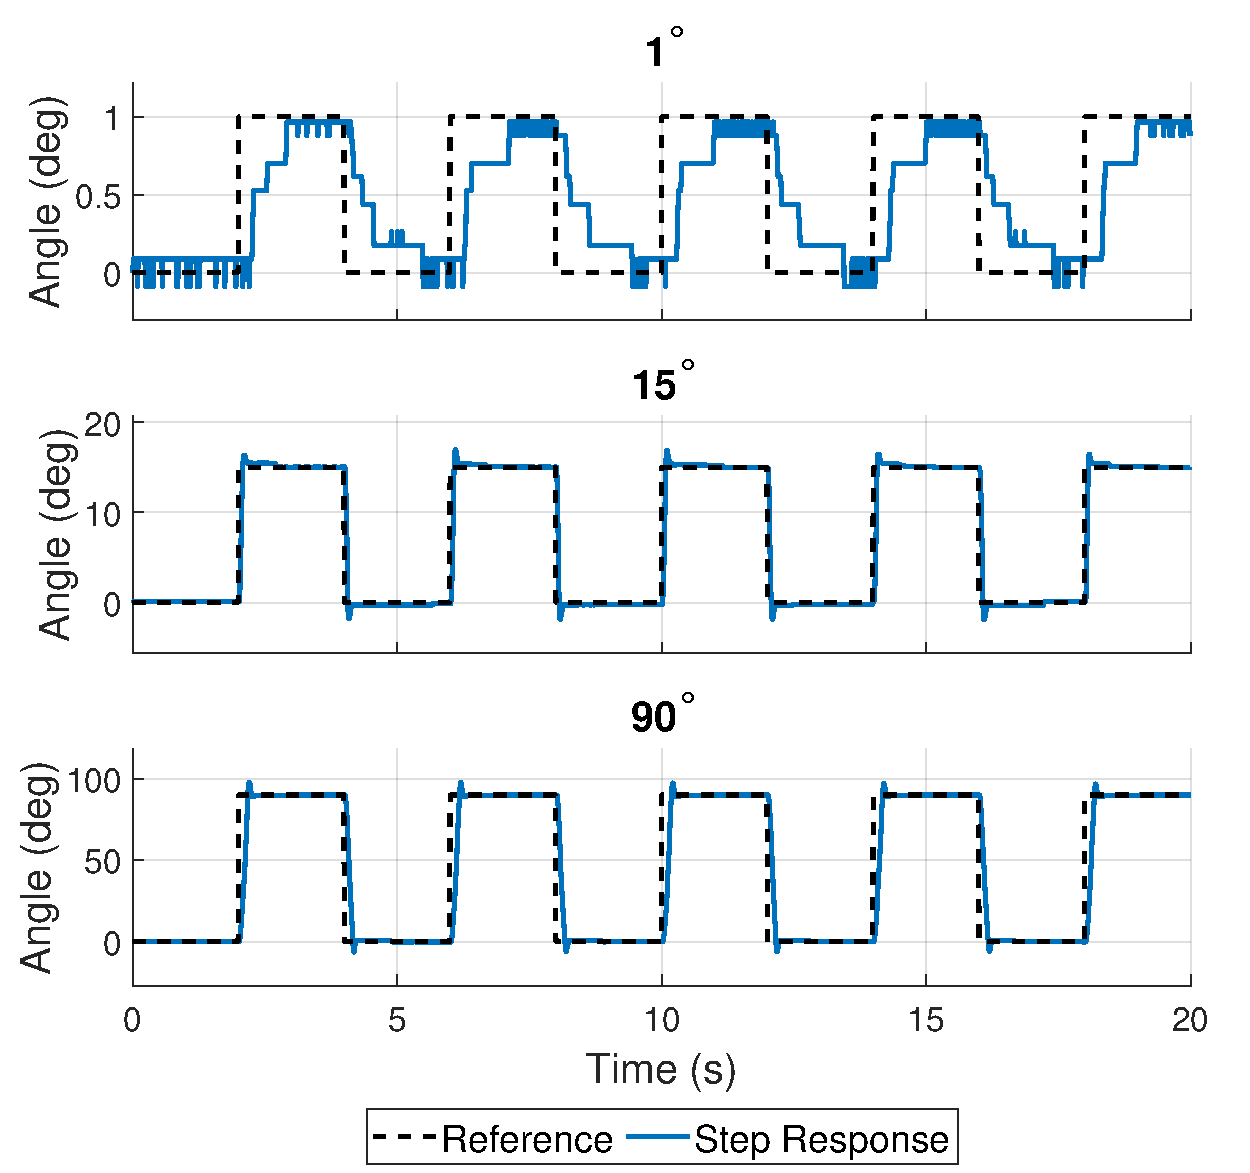
\includegraphics[width=0.98\textwidth]{images/custom_step_response_multi.pdf}
    \caption{Trajectory Tracking}
    \label{fig:step_responses}
\end{figure}

\begin{figure}[htbp]
    \centering
    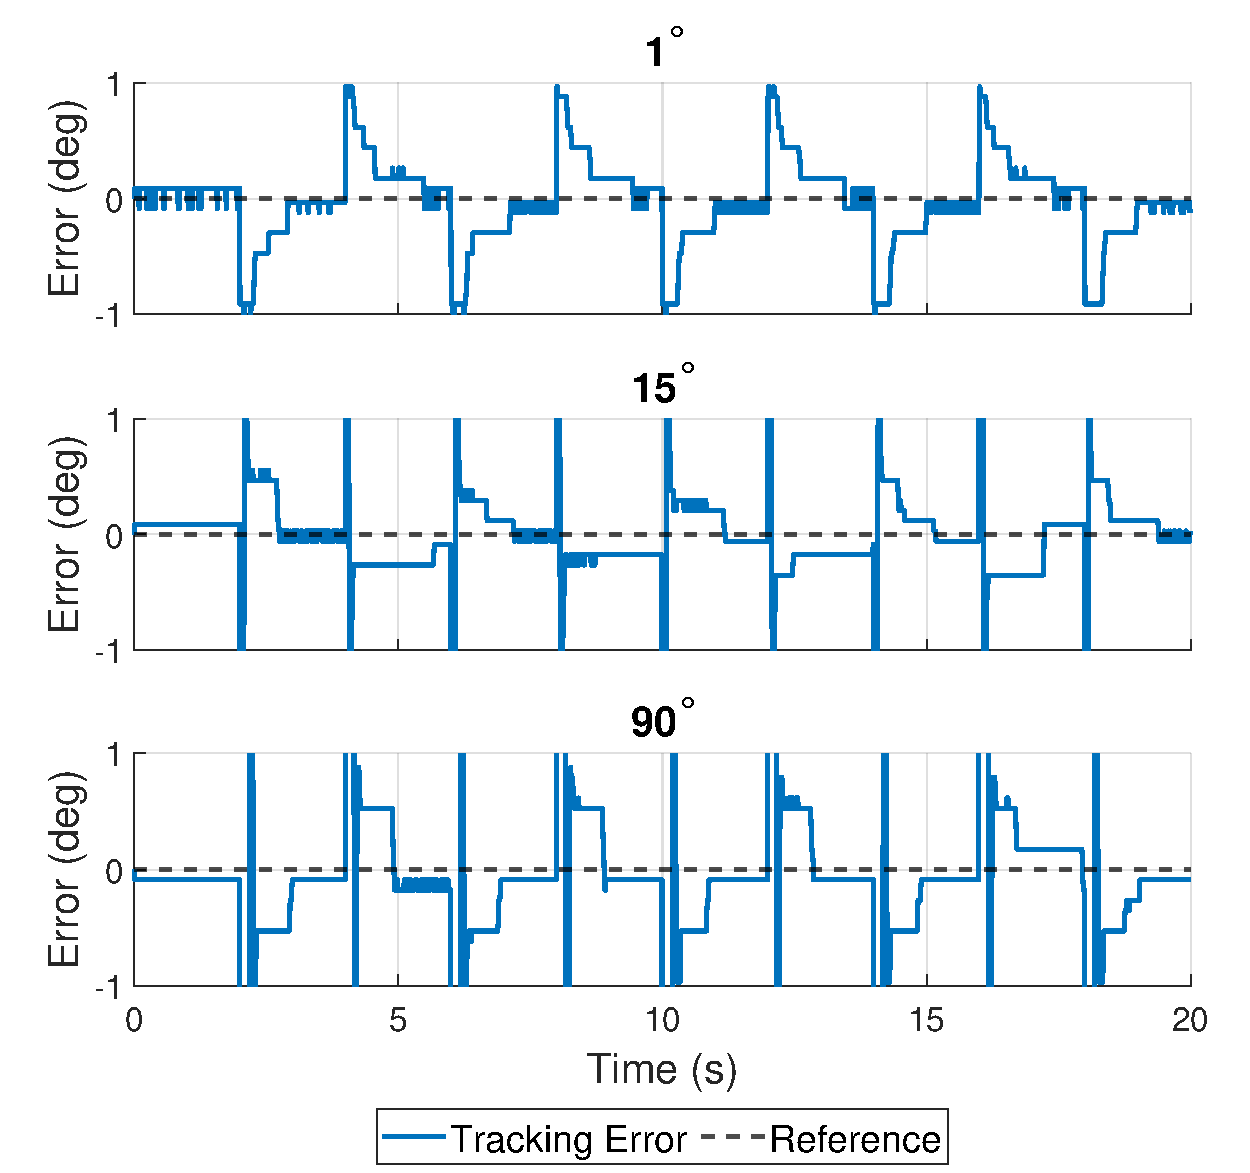
\includegraphics[width=0.98\textwidth]{images/custom_step_error_multi.pdf}
    \caption{Tracking Errors}
    \label{fig:step_error}
\end{figure}


\subsection{Results Summary}

The experimental results confirm that the custom actuator meets the strict requirements of the limb
application. The redesign has yielded a substantial increase in precision, accuracy, and controllability.
The transition to a digital interface ensures scalability and flexibility, while the mechanical form factor
remains compatible with the original design.

To quantify these improvements, a direct benchmark comparison was performed against the two commercial units
characterized in Section \ref{sec:limitations}. Figure \ref{fig:benchmark} illustrates the performance metrics
regarding positioning accuracy and mechanical play.

For the sake of brevity, the mathematical definitions of the metrics used in this analysis (RMSE, Absolute
Error, Hysteresis) are detailed in Appendix \ref{app:metrics}.

\begin{figure}[htbp]
    \centering
    
\includegraphics[width=0.96\textwidth]{images/final_benchmark.pdf}
    \caption{Performance Benchmark Results.}
    \label{fig:benchmark}
\end{figure}

The data reveals a dramatic enhancement in performance:

\begin{itemize}
    \item \textbf{Accuracy:} The Root Mean Square Error (RMSE), which serves as a reliable indicator of
        global linearity and tracking fidelity, dropped from an average of $\approx 14^{\circ}$ in the
        commercial units to just $\mathbf{0.37^{\circ}}$ in the custom prototype. This result comfortably
        satisfies the design requirement of $<\pm 0.5^{\circ}$ set in Section \ref{sec:hardware}.
    \item \textbf{Peak Error:} The Maximum Absolute Error was reduced from extreme values
        ($\approx 29^{\circ}$ for Unit A) to a manageable $\mathbf{1.49^{\circ}}$, effectively eliminating
        the macroscopic non-linearities observed in the analog potentiometers.
    \item \textbf{Hysteresis:} The stick-slip and backlash effects were significantly mitigated. The average
        hysteresis was reduced from $\approx 5^{\circ}$ to $\mathbf{0.65^{\circ}}$, validating the
        effectiveness of the Switching PID strategy in compensating for static friction.
\end{itemize}

Finally, a cost analysis (Appendix \ref{app:bom}) indicates that these performance gains were achieved within
a very limited budget, proving the viability of the proposed custom solution over expensive high-end commercial
alternatives. Further hardware and software improvements can be implemented in the next revision and are left
as future work.



    \chapter{Prototype Implementation}
\label{ch:prototype}

Following the successful design and characterization of the custom actuator module, the research progresses
to the system-level integration. This chapter details the physical assembly of the modular robotic limb and
the establishment of the control infrastructure required to bridge the simulation environment with the real
world.

The primary objective of this phase is to validate the mechanical design and the kinematic control strategies
derived in Chapter \ref{ch:model} under real-world conditions. The validation relies on a
Hardware-in-the-Loop (HIL) architecture, which allows for direct comparison between the theoretical model
and the physical prototype.

The scope of these experiments is strictly limited to the verification of the kinematic model and trajectory tracking
capabilities in an open-loop configuration. The proprioceptive and adaptive control strategies discussed in Section
\ref{sec:proprioception}, while validated in simulation, are excluded from this experimental verification due to
project time constraints.

\section{Hardware-in-the-Loop Architecture}

The successful implementation of the prototype relies on the seamless integration of the mechanical hardware
with the control software. To bridge the theoretical environment (MATLAB/Simulink) with the physical reality, a
Hardware-in-the-Loop (HIL) architecture was established. This approach allows the complex kinematic algorithms
to run on the host PC, while a dedicated embedded bridge manages the low-level communication with the distributed
actuator network.


\subsubsection{Physical Assembly}

The mechanical structure of the limb was realized through additive manufacturing (3D printing) using the CAD
models developed during the design phase. The structural links (Coxa, Femur, Tibia) were printed in PLA to
ensure an optimal stiffness-to-weight ratio.

These components were assembled with the three newly designed custom actuator modules described in Chapter
\ref{ch:servomotor} (see Figure \ref{fig:limb_assembly}). A critical design feature introduced in this assembly is
the axis extension mechanism. To mitigate the radial stress on the servo output shaft an idler bearing was integrated
into the frame opposite to the motor shaft. This configuration effectively creates a simply supported beam structure,
significantly increasing mechanical stability.

\begin{figure}[htbp]
    \centering
    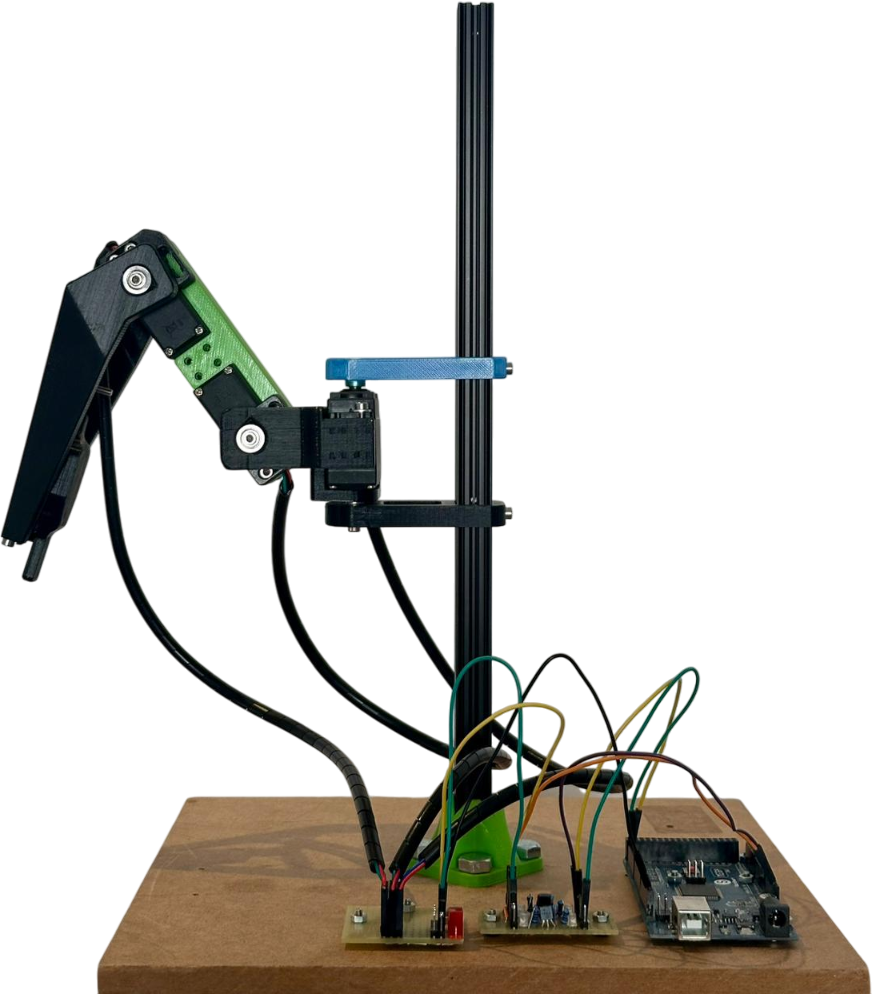
\includegraphics[width=0.88\textwidth]{images/limb_assembly.png}
    \caption{Mechanical Assembly of the Prototype Limb.}
    \label{fig:limb_assembly}
\end{figure}

With the exception of the custom actuator housings and fasteners, the physical limb geometrically coincides perfectly
with the numerical model used in the simulations (Section \ref{sc:simulation}), providing a first visual
confirmation of the prototype's fidelity.


\subsubsection{Simulink/Arduino Control Environment}

The Simulink model, originally developed for pure digital simulation, acts as the High-Level Controller. The
"Leg Model (Plant)" block used in Chapter \ref{ch:model} is replaced by a Serial Interface Block. This modified
control scheme (Figure \ref{fig:hil_scheme}) operates as follows:

\begin{enumerate}
    \item Generation and Transmission: The Path Planner and Inverse Kinematics blocks generate the reference
        joint angles $q_d$ in real-time. These references are quantized and transmitted via USB-Serial to the
        microcontroller bridge.
    \item Hardware Bridge: The interface between the host PC and the actuator network is managed by an Arduino
        board (Arduino Mega 2560). The firmware sketch, parses the UART data and forwards the position setpoints
        to the actuator network via $\text{I}^2\text{C}$ bus. Immediately after it queries their current position
        (also via $\text{I}^2\text{C}$). Then the received data ($q_{hw}$) is transmitted back to Simulink.
    \item Feedback Loop: After the return packet containing the measured joint angles $q_{hw}$ arrives, the
        feedback data is fed into the Forward Kinematics block to reconstruct the actual end-effector position
        $p_{hw}$ for performance analysis.
\end{enumerate}

\begin{figure}[htbp]
    \centering
    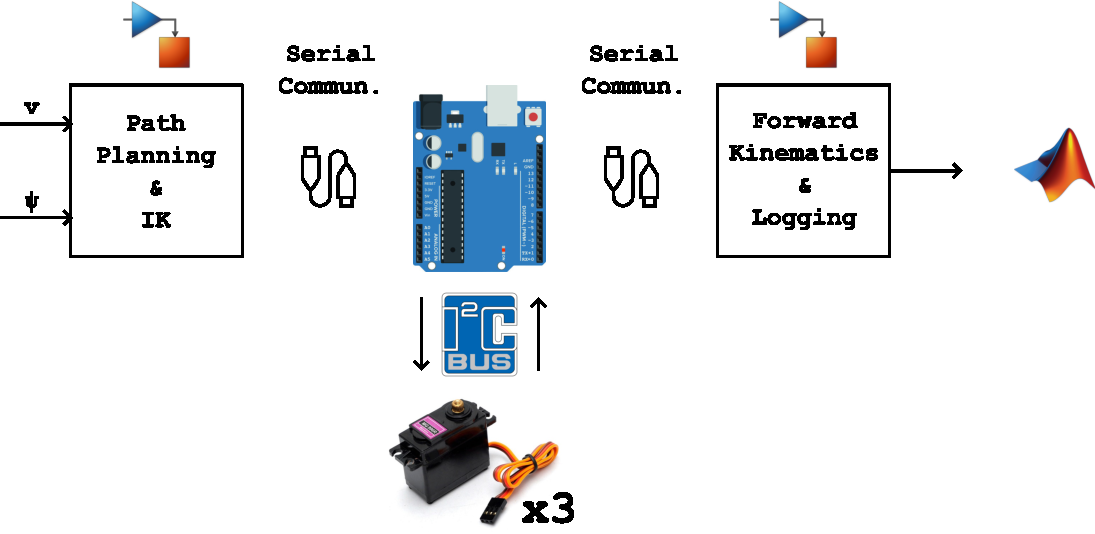
\includegraphics[width=0.9\textwidth]{images/hil.pdf}
    \caption{Block Diagram of the Hardware-in-the-Loop Control Architecture.}
    \label{fig:hil_scheme}
\end{figure}


\subsubsection{Experimental Protocol}

To ensure a rigorous validation, the experimental setup is designed to strictly mirror the conditions of the
digital simulation presented in Chapter \ref{ch:model}. The reference input for the physical limb is the exact
same $C^2$ continuous gait trajectory derived in Section \ref{sec:trajectory}.

The real-time control chain operates at a fixed update frequency of $100\,\text{Hz}$ ($\Delta t = 10\,\text{ms}$).
In each cycle, the Simulink High-Level Controller samples the continuous trajectory, computes the inverse
kinematics solution $q_d$, and transmits the packet to the embedded bridge. Synchronously, the actual joint
positions $q_{hw}$ are acquired from the actuators and logged.

The primary objective of this experiment is to quantify the \textit{Sim-to-Real} gap by overlaying the
experimental data on the simulation results.
\section{Performance Assessment and Results}

The following results provide a quantitative comparison between the reference command ($p_d$, $q_d$), the
simulated response ($p_{sim}$, $q_{sim}$), and the actual experimental telemetry ($p_{hw}$, $q_{hw}$).


\subsubsection{Cartesian Trajectory Tracking}

Figure \ref{fig:gait_z_psi_exp} illustrates the side-view trajectory ($Z\psi$-plane) of the end-effector. Visual
inspection confirms that the physical limb successfully replicates the desired gait profile. The stance phase remains
reasonably flat, while the swing phase achieves the target clearance height without significant deviation. Crucially,
the experimental path (orange) remains close to the Optimal Workspace Region (dotted line), validating the
safety margins established during the design phase.

\begin{figure}[htbp]
    \centering
    
\includegraphics[width=0.65\textwidth]{images2/gait_z_psi.pdf}
    \caption{Experimental Gait Trajectory in the $Z\psi$-plane (Side View).}
    \label{fig:gait_z_psi_exp}
\end{figure}

Figure \ref{fig:gait_spacetime} shows the time evolution of the trajectory in a 3D graph. Several persistent
perturbations can be seen along the path. This is attributed to model calculation lags on the simulink side,
as they appear during the FSM path generator state transition, and also to external force (gravity).

\begin{figure}[htbp]
    \centering
    
\includegraphics[width=0.65\textwidth]{images2/gait_3d_spacetime.pdf}
    \caption{Experimental Gait Trajectory in Space-Time.}
    \label{fig:gait_spacetime}
\end{figure}

A time-domain analysis of the Cartesian coordinates is provided in Figure \ref{fig:cart_traj_exp}. The experimental
tracking shows a high degree of fidelity, with all the coordinates closely following the command. The $X$ coordinate,
which should ideally remain constant, shows minor fluctuations ($< 2$ mm) negligible for locomotion stability, while
the $Y$ (propulsion) and $Z$ (lift) components exhibit a small tracking delay. This is expected due to the discrete
nature of the control loop.

\begin{figure}[htbp]
    \centering
    \begin{subfigure}[b]{0.8\textwidth}
        \centering
        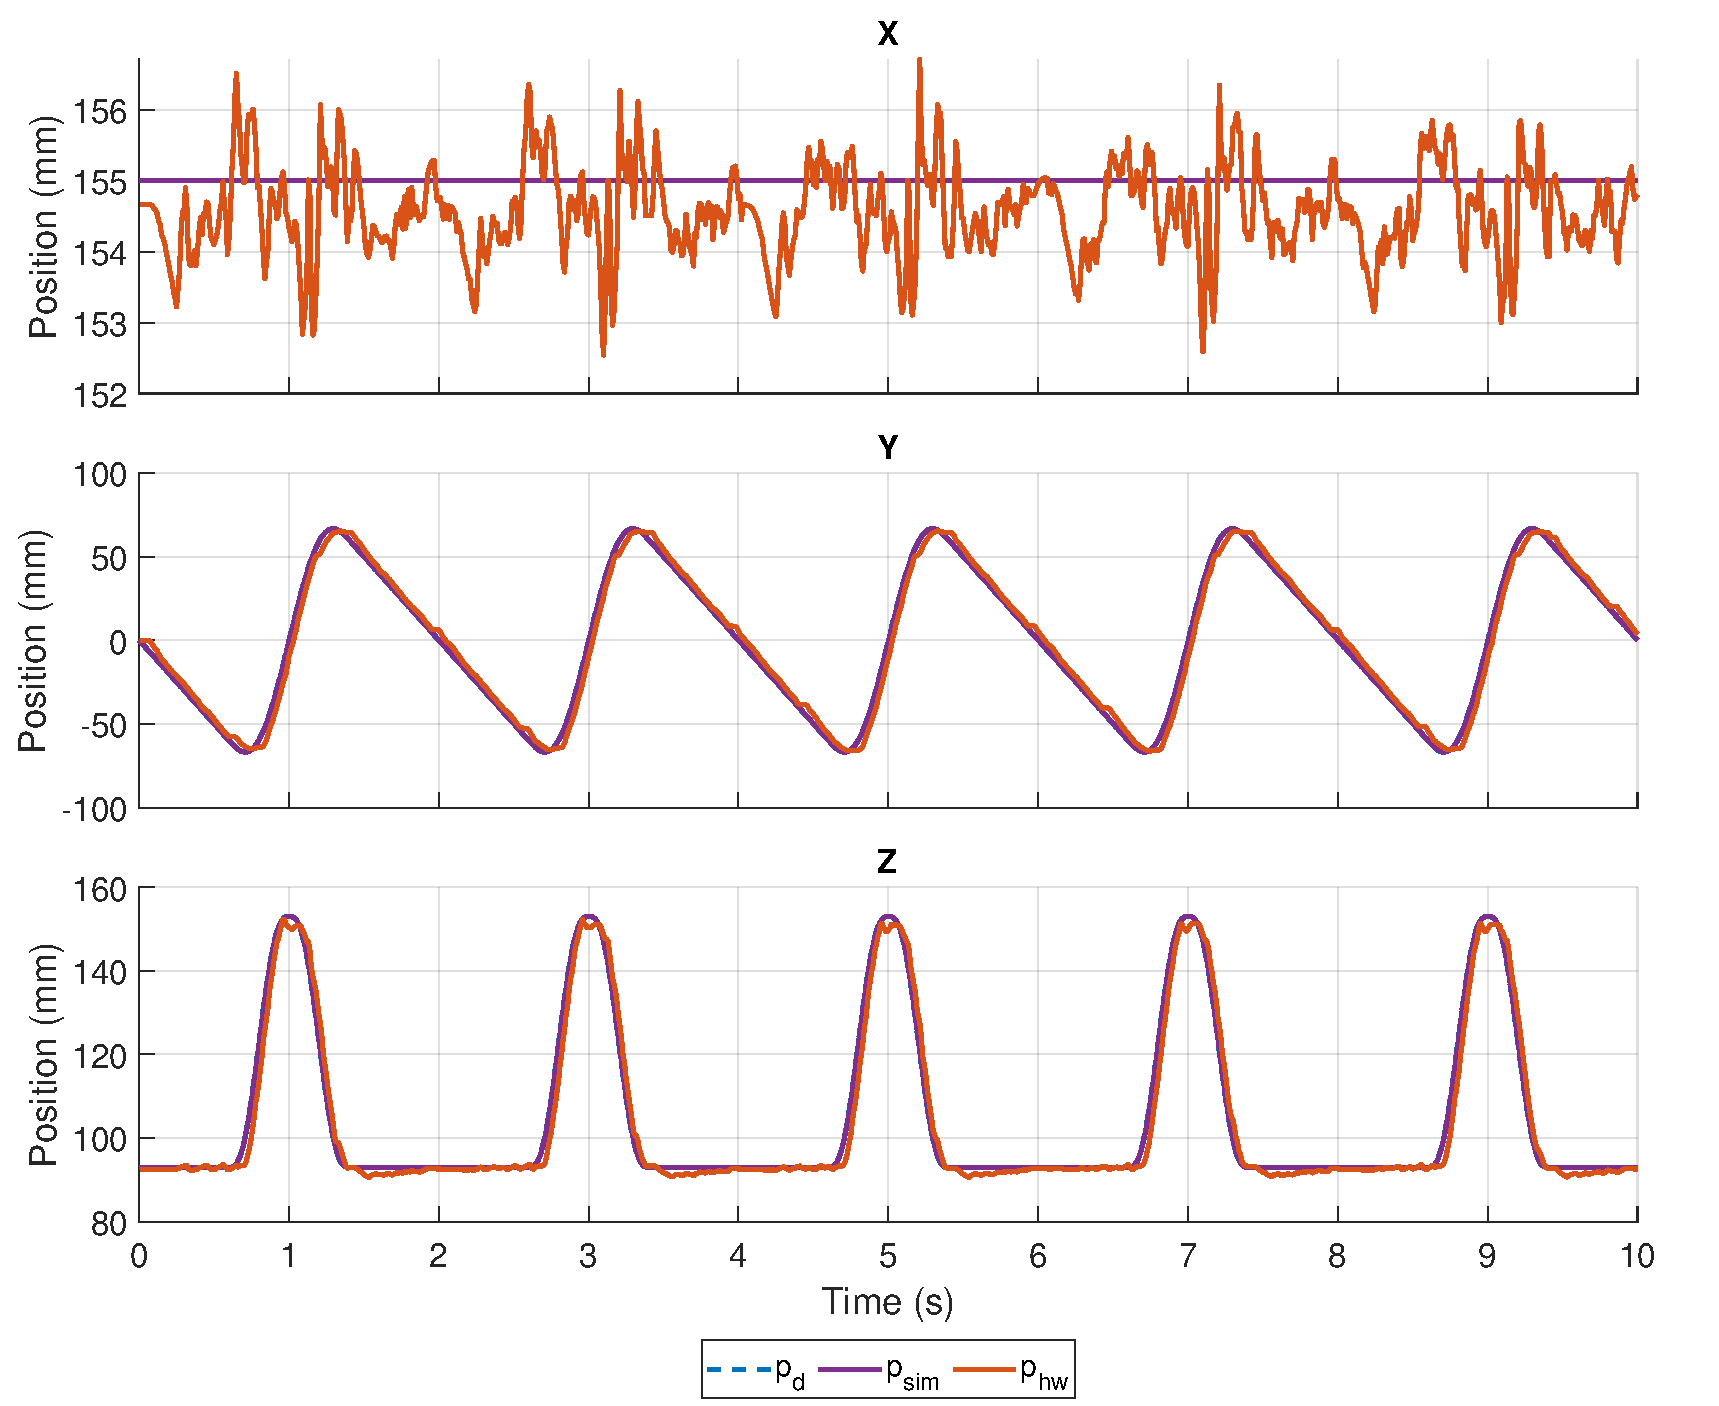
\includegraphics[width=\textwidth]{images2/cartesian_trajectories.pdf}
        \caption{Trajectory Tracking}
        \label{fig:cart_traj_exp}
    \end{subfigure}

    \begin{subfigure}[b]{0.8\textwidth}
        \centering
        
\includegraphics[width=\textwidth]{images2/cartesian_errors.pdf}
        \caption{Tracking Errors}
        \label{fig:cart_err_exp}
    \end{subfigure}
    \caption{Cartesian-Space Experiment Results.}
    \label{fig:cart_exp}
\end{figure}

The error plot (Figure \ref{fig:cart_err_exp}) reveals similarities in the simulation and experimental error shapes,
fundamentally changing only in amplitude (refer also to Figure \ref{fig:joint_results} for better understanding).
The amplitude difference can be attributed to a higher tracking delay, while the shape of the error is reasonably
due to inertial effects, purposely neglected at this stage of control.


\subsubsection{Joint Space Performance}

The performance at the actuator level is detailed in Figures \ref{fig:joint_traj_exp} and \ref{fig:joint_err_exp},
where once again it is visible how all three joints ($q_1, q_2, q_3$) track their respective references with
remarkable precision (also in this instance, the Simulation and Experimental plots differ by amplitude rather than
shape).

\begin{figure}[htbp]
    \centering
    \begin{subfigure}[b]{0.8\textwidth}
        \centering
        
\includegraphics[width=\textwidth]{images2/joint_trajectories.pdf}
        \caption{Trajectory Tracking}
        \label{fig:joint_traj_exp}
    \end{subfigure}

    \begin{subfigure}[b]{0.8\textwidth}
        \centering
        
\includegraphics[width=\textwidth]{images2/joint_errors.pdf}
        \caption{Tracking Errors}
        \label{fig:joint_err_exp}
    \end{subfigure}
    \caption{Joint-Space Experiment Results.}
    \label{fig:joint_exp}
\end{figure}


\subsubsection{Delay and Response Analysis}

To isolate the dynamic performance from the temporal evolution to promote a better visualization of the mentioned
tracking delay, Figure \ref{fig:tracking_delay_exp} presents the input-output correlation (Command vs. Measured
angle) for each joint. An ideal behaviour should be represented by a straight line ($y = x$), while a wider ellipse
would correspond to a higher tracking delay.

Both datasets populates the graph as expected (narrow ellipses for simulation and wider ellipses for the experiment).
Additionally, the slightly wider loops for $q_2$ and $q_3$ correlate with a higher inertial load due to gravity.

\begin{figure}[htbp]
    \centering
    \begin{subfigure}[b]{0.40\textwidth}
        \centering
        
\includegraphics[width=\textwidth]{images2/q_track_1.pdf}
        \caption{Hip ($q_1$)}
    \end{subfigure}
    \begin{subfigure}[b]{0.40\textwidth}
        \centering
        
\includegraphics[width=\textwidth]{images2/q_track_2.pdf}
        \caption{Knee ($q_2$)}
    \end{subfigure}

    \begin{subfigure}[b]{0.40\textwidth}
        \centering
        
\includegraphics[width=\textwidth]{images2/q_track_3.pdf}
        \caption{Ankle ($q_3$)}
    \end{subfigure}
    \caption{Tracking Delay Analysis.}
    \label{fig:tracking_delay_exp}
\end{figure}


\subsubsection{Quantitative Benchmark}

Unexpectedly, the tracking quality performs surprisingly well, despite the fact that the custom servomotor control
algorithm is originally designed for P2P control.

Ultimately, the tracking quality is quantified using the Root Mean Square Error (RMSE) metric (as per Section
\ref{sec:limitations}). Figure \ref{fig:rmse_benchmark} compares the simulation baseline against the physical
prototype.

While the experimental errors are naturally higher than the idealized simulation, the general trend matches for the
two cases, following similar magnitude patterns. The Cartesian RMSE is dominated by the Y-axis ($\approx 5.4$ mm),
consistent with the direction of maximum movement and backlash accumulation.
The main contributor to these errors in the experimental case, as shown in the previous section, was the tracking
delay. Nevertheless, the error remains however remarkably small for a low-cost prototype.

This quantitative benchmark conclusively validates the design approach: the custom actuators and the kinematic
model perform within the requirements defined at the outset of this thesis and well within acceptable limits for
stable locomotion.

\begin{figure}[htbp]
    \centering
    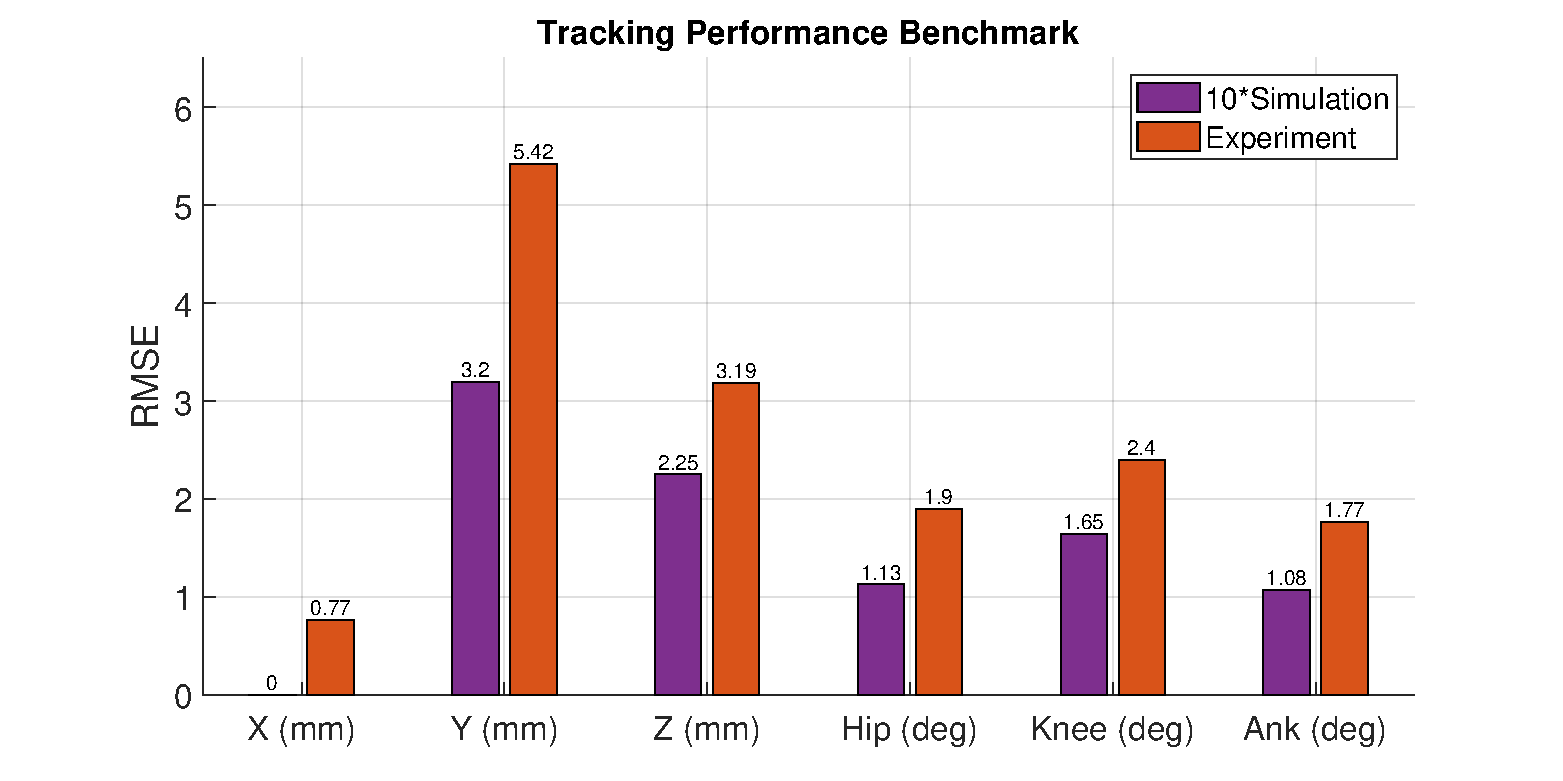
\includegraphics[width=0.98\textwidth]{images/rmse_benchmark.pdf}
    \caption{Simulation vs. Experiment Tracking Error.}
    \label{fig:rmse_benchmark}
\end{figure}

    \chapter{Conclusions}
\label{ch:conclusions}

This thesis has documented the complete engineering cycle of a modular robotic limb, moving from the theoretical
kinematic analysis to the physical realization of a high-performance, cost-effective actuation system. The central
challenge addressed in this work was the "actuation bottleneck" typical of low-cost robotics, where the mechanical
and control performance is severely limited by the poor quality of commercial hobbyist servo-motors. By adopting a
top-down design methodology, supported by simulation and component-level redesign, this research successfully
demonstrated that high-fidelity control can be achieved without resorting to prohibitively expensive industrial
hardware.


\section{Achievements and Considerations}

The primary technical achievement of this work is the development and validation of the custom "Smart Actuator" module.
The transition from a standard analog architecture to a fully digital, microcontroller-based system yielded quantifiable
improvements in every key performance metric.

As demonstrated by the experimental benchmarking in Chapter \ref{ch:servomotor}, the custom module reduced the Root
Mean Square Error (RMSE) in position tracking from an average of $\approx 14^{\circ}$ (observed in the original MG996R
units) to just $0.37^{\circ}$. This result confirms that the limitations of low-cost robotics are often not mechanical
but electronic and algorithmic. Specifically:

\begin{itemize}
    \item \textbf{Linearity and Precision:} The integration of the AS5600 magnetic encoder eliminated the
        non-linearities and wear associated with resistive potentiometers, providing a stable 12-bit feedback
        signal.
    \item \textbf{Friction Compensation:} The implementation of the Switching PID control strategy proved effective in
        mitigating the stick-slip phenomenon. The ability to dynamically switch integrator states allowed the actuator
        to overcome static friction without inducing the limit-cycle oscillations (hunting) typical of standard linear
        controllers.
    \item \textbf{Sim-to-Real Fidelity:} The Hardware-in-the-Loop validation detailed in Chapter \ref{ch:prototype}
        confirmed a high degree of correlation between the Simulink numerical model and the physical prototype.
\end{itemize}


\section{Economical and Practical Aspects}

From an economical perspective, the custom module represents a strategic compromise between cost and performance.
Industrial actuators capable of similar precision typically cost between 10 to 20 times more than a standard hobby
servo. The prototype developed in this thesis achieves comparable tracking fidelity at a fraction of that cost,
maintaining a bill of materials (BOM, Appendix \ref{app:bom}) compatible with academic and hobbyist budgets.

A crucial practical advantage of this design is its retro-compatibility. By strictly adhering to the external
form factor of the standard "40x20x36mm" servo case, the custom module acts as a "drop-in replacement". This allows for
the immediate upgrade of existing hexapod platforms without requiring any mechanical redesign or the re-printing of
structural parts. Furthermore, the shift to an $I^2C$ bus architecture simplifies the robot's wiring harness, allowing
multiple actuators to be daisy-chained on a single cable, thereby reducing the complexity and weight of the central
electronics.


\section{General Applicability and Future Work}

While this research focused on a hexapod limb, the developed "Smart Actuator" has general applicability across the field
of robotics. It can be effectively employed in low-cost robotic arms, camera gimbals, or bipedal systems where precision
and customizability are required but budget is constrained.

However, several areas remain open for future development to transition from this single-leg prototype to a fully
autonomous hexapod robot:

\begin{itemize}
    \item \textbf{Proprioceptive Validation:} The adaptive "Blind Walking" strategy and the Finite State Machine
        trajectory generator were validated only in the simulation environment (Chapter \ref{ch:model}). Future work
        must focus on enabling the impact detection logic on the physical hardware, utilizing the motor current feedback
        or external contact sensors to handle uneven terrain.
    \item \textbf{Dynamic Tuning Optimization:} The PID gains used in the experimental validation were tuned empirically.
        Implementing an auto-tuning routine or a model-based parameter identification algorithm would further optimize
        the controller's response to varying loads.
    \item \textbf{Full-Body Integration:} The final step is the replication of the limb design to assemble the complete
        hexapod. This will introduce new challenges regarding power management, inter-leg coordination, and the global
        stability of the chassis, which were outside the scope of this single-leg study.
\end{itemize}

In conclusion, this thesis lays a solid foundation for the development of accessible, high-performance legged robots,
proving that intelligent control design can effectively bridge the gap between low-cost hardware and advanced robotic
capabilities.
    \chapter*{Declaration on the Use of Generative AI}
\addcontentsline{toc}{chapter}{Declaration on the Use of Generative AI}

In accordance with the guidelines for the responsible use of AI, the author acknowledges the use of Generative AI tools
(specifically Google Gemini) to assist with English language proofreading, sentence structure optimization, and the
drafting and debugging of the embedded firmware code.

The author certifies that the conceptual design and scientific core of the thesis, including the mechanical design of
the hexapod limb, the custom PCB design, and the interpretation of experimental results, are the result of the author's
original work.

All content and code segments generated or suggested by AI tools were subjected to a rigorous critical review and
verification by the author to ensure accuracy and compliance with the project specifications. The author bears full
responsibility for the final content of this thesis.


\chapter*{Ringraziamenti}
\addcontentsline{toc}{chapter}{Ringraziamenti}

Chi mi conosce sa che solitamente preferisco esprimere affetto o gratitudine attraverso gesti piuttosto che a parole.
Molto spesso la causa è la vergogna o l'imbarazzo, che mi fanno sentire vulnerabile, ma per questa occasione ho deciso
di fare uno sforzo.

Un grazie speciale ai miei genitori, Enzo e Manuela, da sempre i miei sostenitori numero 1. Mi sopportano dal mio primo
giorno di vita (un lavoro molto duro, ne sono consapevole). Sappiate che anche se non sono bravo a farvelo capire, vi
voglio un mondo di bene e vi porterò sempre nel mio cuore.

Ringrazio mia sorella Annalaura, che seppur controvoglia, alla fine si impegna sempre per darmi una mano quando serve.

Ringrazio Letizia, la mia compagna, con cui ormai da anni condivido passioni ed avventure. Sono sicuro che il futuro ci
riserverà molti altri momenti speciali.

Ringrazio Mattia, Linda e Marco M., i miei migliori amici. Con voi riesco sempre ad essere felice e abbandonare ogni
preoccupazione, anche nei momenti più bui.

Grazie a tutti gli amici, che negli anni mi hanno accompagnato, tra alti e bassi. In particolare il gruppo del Fantabosco,
(Max, Matteo B., Lucrezia, Fra e Daniel) con cui ho condiviso serate indimenticabili, gli ultimi arrivati dell'università
(Gio, Giulia, Liuk, Fede, Paolo, Anna, Edo, Noemi, Mary, RKB ed Elena) con cui sono sopravvissuto tra un esame e l'altro,
a questi ultimi tre anni, ma anche il gruppo della laurea triennale (Marco L., Matteo V., Tomas, Marta e Bias).
Tutti voi, sappiate che anche se dovessimo non rimanere più in contatto, da parte mia sarà come non avervi mai salutati,
e se avrete bisogno di aiuto saprete dove trovarmi.

Un sentito ringraziamento anche al Professor Angelo Cenedese, che mi ha permesso di proseguire questo progetto personale
fino a qui, mostrandosi da subito molto disponibile.

Infine, ringrazio chiunque abbia mai incrociato il suo cammino con il mio, nel bene e nel male. Sono convinto che senza
anche uno solo di voi, non sarei la persona che oggi sono fiero di essere.
    \cleardoublepage

    % --- APPENDICI ---
    \appendix
    \chapter{Appendix}

\newpage
\section{Full Inverse Kinematics Expressions}
\label{app:ik}

{\footnotesize\begin{align}
    q_1 &= \operatorname{atan2}(y_d, x_d)
    \\[3ex]
    q_2 &= \operatorname{acos}\left(\frac{a_2^2 - a_3^2 + \left(\sqrt{x_d^2 + y_d^2} - a_1\right)^2 + (d_b - z_d)^2}
    {2 \cdot a_2 \cdot \sqrt{\left(\sqrt{x_d^2 + y_d^2} - a_1\right)^2 + (d_b - z_d)^2}}\right) -
    \operatorname{atan2}\left((d_b - z_d), \left(\sqrt{x_d^2 + y_d^2} - a_1\right)\right)
    \\
    q_3 &= \operatorname{acos}\left(\frac{a_2^2 + a_3^2 - \left(\sqrt{x_d^2 + y_d^2} - a_1\right)^2 - (d_b - z_d)^2}
    {2 \cdot a_2 \cdot a_3}\right)
    \label{eqn:inverse_kinematics}
\end{align}}


\newpage
\section{Servo Module Schematic}
\label{app:pcb}

\begin{figure}[htb]
    \centering
    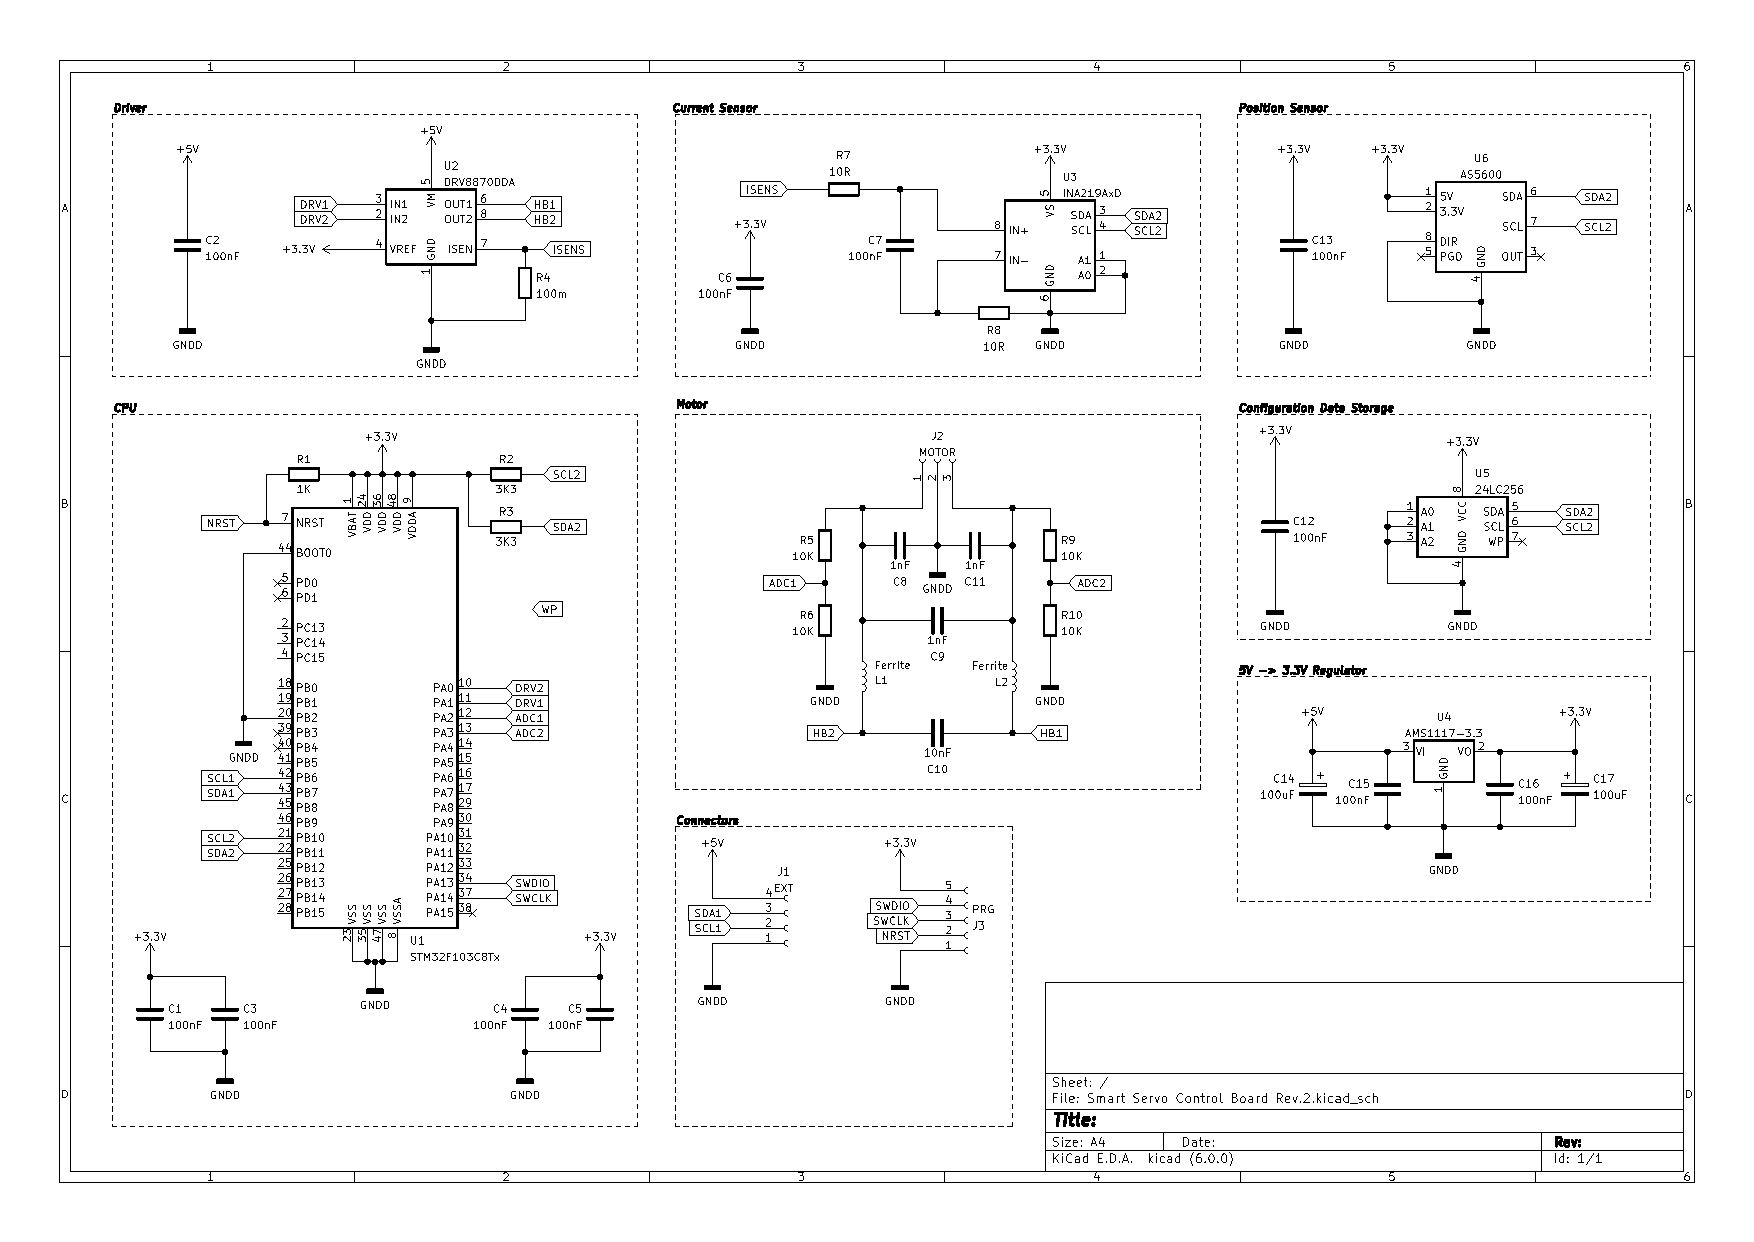
\includegraphics[angle = 90, width=0.8\textwidth]{images/schematic.pdf}
\end{figure}


\newpage
\section{Software Architecture}
\label{app:software}

\begin{figure}[htb]
    \centering
    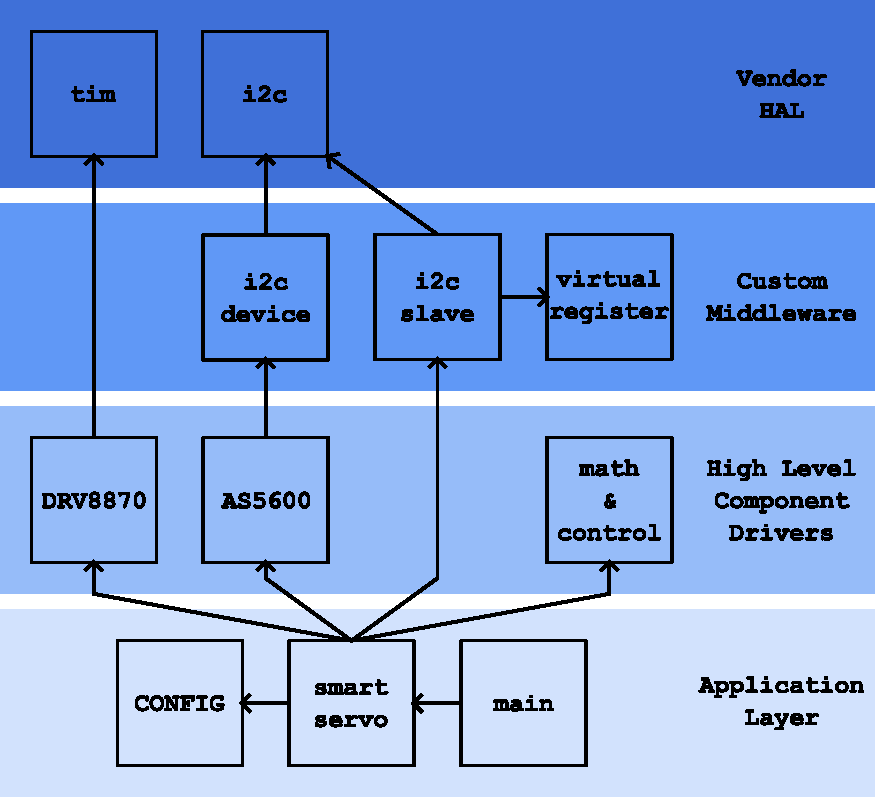
\includegraphics[width=\textwidth]{images/software_architecture.pdf}
\end{figure}


\newpage
\section{Register Map}
\label{app:register}

\begin{longtable}{@{} l l l l l @{}}
\caption{System Register Map} \\

% --- Intestazione Prima Pagina ---
\toprule
\textbf{Addr} & \textbf{Register Name} & \textbf{Data Type} & \textbf{Group} & \textbf{Default} \\
\midrule
\endfirsthead

% --- Intestazione Pagine Successive ---
\toprule
\textbf{Addr} & \textbf{Register Name} & \textbf{Data Type} & \textbf{Group} & \textbf{Default} \\
\midrule
\endhead

% --- Footer Pagine Intermedie ---
\midrule
\multicolumn{5}{r}{\textit{Continued...}} \\
\bottomrule
\endfoot

% --- Footer Finale ---
\bottomrule
\endlastfoot

% --- CONTENUTO ---

% SW-PID Controller (Tipi dedotti da DefaultSettings: float)
\texttt{0x00} & ProportionalGain   & \texttt{float}    & SWPID Control & $10.0f$ \\
\texttt{0x01} & IntegralGain       & \texttt{float}    & SWPID Control & $0.9f$ \\
\texttt{0x02} & DerivativeGain     & \texttt{float}    & SWPID Control & $0.1f$ \\
\texttt{0x03} & AntiwindupMax      & \texttt{float}    & SWPID Control & $5.0f$ \\
\texttt{0x04} & AntiwindupMin      & \texttt{float}    & SWPID Control & $-5.0f$ \\
\texttt{0x05} & OutputMax          & \texttt{float}    & SWPID Control & $1.0f$ \\
\texttt{0x06} & OutputMin          & \texttt{float}    & SWPID Control & $-1.0f$ \\
\addlinespace

% Servo Motor State (Non presenti in Default, ipotizzo float per coerenza)
\texttt{0x20} & DesiredPosition    & \texttt{int32\_t}  & Servo State & 0 \\
\texttt{0x21} & ActualPosition     & \texttt{int32\_t}  & Servo State & - \\
\texttt{0x22} & PositionOffset     & \texttt{int32\_t}  & Servo State & -2048 \\
\texttt{0x26} & DutyCycle          & \texttt{int32\_t}  & Servo State & - \\
\addlinespace

% AS5600 (Tipi dedotti: uint16_t)
\texttt{0x40} & ZeroPosition       & \texttt{uint16\_t} & AS5600     & \texttt{0x000} \\
\texttt{0x41} & StopPosition       & \texttt{uint16\_t} & AS5600     & \texttt{0xFFF} \\
\addlinespace

\end{longtable}


\newpage
\section{Metrics Formulae}
\label{app:metrics}

\textbf{Root Mean Square Error (RMSE)}
$$\text{RMSE} = \sqrt{ \frac{1}{N} \sum_{i=1}^{N} \left( y_{meas}[i] - y_{ideal}[i] \right)^2 }$$

This metric quantifies the standard deviation of the residuals between the measured output ($y_{meas}$) and the ideal
theoretical reference ($y_{ideal}$). It serves as the primary indicator of the system's overall linearity accuracy,
aggregating the error over the entire dataset.


\textbf{Maximum Absolute Error}
$$E_{max} = \max_{i} \left| y_{meas}[i] - y_{ideal}[i] \right|$$

Represents the worst-case deviation observed across the entire operating range. It identifies the single instance
where the actuator's position diverged most significantly from the expected ideal value.


\textbf{Hysteresis Loop Area}
$$\mathcal{A}_{hyst} = \left| \int_{x_{min}}^{x_{max}} \left( y_{fwd}(x) - y_{bwd}(x) \right) \, dx \right|$$

Calculated via numerical integration (trapezoidal rule), this value represents the total area enclosed between the
forward ($y_{fwd}$) and backward ($y_{bwd}$) trajectories. It quantifies the cumulative effect of mechanical backlash,
friction, and sensor noise over a full motion cycle.


\textbf{Average Hysteresis Error}
$$H_{avg} = \frac{\mathcal{A}_{hyst}}{x_{max} - x_{min}}$$

This metric normalizes the hysteresis area by the input signal range ($x_{max} - x_{min}$). It provides the average
magnitude of the hysteresis gap in degrees, allowing for a direct and fair comparison between systems operating on
different input domains.


\newpage
\section{Bill of Material}
\label{app:bom}

Bill of Materials (BOM) for a single custom actuator module. Prices reflect the per-unit cost derived from bulk purchases
on third-party websites and are comprehensive of shipping.

\begin{table}[htbp]
    \centering
    \begin{tabular}{lccc}
        \toprule
        \textbf{Component}  & \textbf{Qty} & \textbf{Bulk Price Reference} & \textbf{Unit Cost (€)} \\
        \midrule
        Custom PCB                              & 1             & 6.18€ / 10 pcs    & 0.62 \\
        STM32F103C8T6 (MCU)                     & 1             & 7.99€ / 10 pcs    & 0.80 \\
        AS5600 (Magnetic Sensor)                & 1             & 4.42€ / 5 pcs     & 0.88 \\
        DRV8870 (Motor Driver)                  & 1             & 2.20€ / 10 pcs    & 0.22 \\
        Tantalum Cap. (100 $\mu$F)              & 2             & 1.47€ / 10 pcs    & 0.29 \\
        AMS1117 (LDO Regulator)                 & 1             & 2.16€ / 50 pcs    & 0.04 \\
        SMD Passives (0603 R/C)                 & $\approx$30   & Lump sum          & 0.25 \\
        MG996R Servo Motor\textsuperscript{*}   & 1             & 20.39€ / 5 pcs    & 4.08 \\
        \midrule
        \textbf{Total Cost per Module} & & & \textbf{7.18} \\
        \bottomrule
    \end{tabular}
    \vspace{1ex}

    {\footnotesize \textsuperscript{*}Current market price (2025). Using older stock (2018), the motor unit cost was
    $\approx 1.92$€, lowering the total to $\approx 5.02$€.}
\end{table}


    % --- BIBLIOGRAFIA ---
    \printbibliography[heading = bibintoc, title = {References}]

\end{document}